%% main_paper_NN42.tex
%% MDPI MAKE 投稿用日本語草稿
%% 入力データの内在次元に基づく AE/VAE ボトルネック次元の選定（版42）
%% 版42の変更点：Peer_Review_Report41.md（Minor to Moderate Revisions）への対応
%%   - 【Major 2】Fashion-MNIST Step 3 を 3 シード検証に格上げ（Exp-Fashion-MS，300 ep）
%%   - 【Major 2】Exp-ConvV-HiBeta を 3 シード検証に格上げ（Exp-ConvV-HiBeta-MS）
%%   - 【Major 1】自然画像で潜在幾何の歪みが顕著になる理由の仮説
%%     （多様体の絡み合い・階層的潜在構造の必要性）を §5.6.2・§6.4 に追加
%%   - 【Major 3】aggregated posterior 不一致 KL(q(z)||p(z)) の非線形最適化中の
%%     挙動に関する考察を注意2・付録 A.1 に追加（ELBO surgery を引用に追加）
%%   - 【Minor 1】要旨から詳細数値を削り，閉ループプロトコルの強調に比重を移す
%%   - 【Minor 2】図2（E4_300ep_multiseed）・図5（Exp_ConvV_HiBeta）を
%%     白黒印刷・縮小に耐える線種・フォントで再生成
%%   - 【Minor 3】Step 2 の乗数 2 が未知の d_emb に対するバッファである旨を再強調
%% ---- 以下は版41の変更点（Review_codex40.txt への対応）----
%%   - §2 の DANCo 記述の矛盾を修正：主推定量には用いないが，MNIST 潜在表現上の
%%     補助的クロスチェックとして使用（Minor 1）
%%   - 参考文献（全引用・引用順番号）と図表の本文言及の全数監査
%% ---- 以下は版40の変更点（Review_codex39.txt への対応）----
%%   - §5 冒頭の実データ検証の設問を「MNIST でプロトコル全体が機能するか，
%%     Fashion-MNIST ではどこまでの証拠が得られるか」に修正（Minor 1）
%%   - リポジトリ URL/DOI（Minor 2）・MDPI プレースホルダ（体裁 1）は
%%     投稿・編集段階で解決（据え置き）
%% ---- 以下は版39の変更点（Review_codex38.txt への対応）----
%%   - §5.3.6 Fashion-MNIST の矛盾文（「フルプロトコルの多シード適用は…
%%     単一シードの予備観察で確認」）を書き直し：Step 1 は多シード，
%%     VAE 側 AU 検証は単一シードの予備観察と明確化（Minor 1）
%%   - §5 冒頭の多シード文を「主判定に用いる VAE 検証結果」に精密化し，
%%     本文中の探索的単一シード要約（高β Conv-VAE・Fashion）に言及（Minor 2）
%%   - MNIST Step 2 に「AE 窓＝TwoNN–MLE 包絡；VAE の m_ver＝主 TwoNN 規則」の
%%     括弧注を追加（Minor 3）
%%   - §1.2 の貢献主張を「MNIST での多シード AU 検証＋Step 1 安定性は
%%     サブサンプリング CI・推定量クロスチェック・3シード参照モデル比較で裏づけ」に
%%     精密化（Minor 4）
%%   - V2 不変域の表示は保守的丸め（平均側の下端は 2.24）と注記（体裁 2）
%%   - 自然画像表キャプションの Pope ら整合を CIFAR-10 限定に（体裁 3）
%%   - 要旨の境界事例記述を軽く圧縮（体裁 4）
%%   - MDPI プレースホルダ（日付・記事番号・DOI・ORCID）は編集段階で解決（体裁 1）
%% コンパイル: platex main_paper_NN42.tex && platex main_paper_NN42.tex && dvipdfmx main_paper_NN42.dvi
%% （参考文献は本文内 thebibliography のため bibtex 不要）

\documentclass[11pt,a4paper]{jsarticle}

\usepackage{amsmath,amsthm,amssymb}
\usepackage{mathtools}
\usepackage[dvipdfmx]{graphicx}
\usepackage{booktabs}
\usepackage{url}
\usepackage{here}
\usepackage{array}
\usepackage{multirow}
\usepackage{enumerate}
\usepackage[margin=25mm]{geometry}
\usepackage[dvipdfmx,hidelinks]{hyperref}
\usepackage{caption}

%% 定理環境
\newtheorem{theorem}{定理}
\newtheorem{proposition}{命題}
\newtheorem{definition}{定義}
\newtheorem{remark}{注意}
\newtheorem{corollary}{系}

%% 記号略記
\newcommand{\dID}{d_{\mathrm{ID}}}
\newcommand{\hatdID}{\hat{d}_{\mathrm{ID}}}
\newcommand{\dz}{m}
\newcommand{\dtrue}{d_{\mathrm{true}}}
\newcommand{\Jg}{J_g}
\newcommand{\R}{\mathbb{R}}
\newcommand{\kap}{\kappa}
\newcommand{\AUsat}{\mathrm{AU}_{\mathrm{sat}}}
\newcommand{\demb}{d_{\mathrm{emb}}}
\newcommand{\mknee}{m^{\mathrm{knee}}}
\newcommand{\dstar}{d^{*}(\beta)}

%% ===================================================================
\title{入力データの内在次元に基づく AE/VAE ボトルネック次元の選定：\\
ID 誘導型プロトコルと Active-Unit 検証}
%% 英語タイトル候補：
%%   Choosing the Bottleneck Dimension of Autoencoders and Variational
%%   Autoencoders from the Intrinsic Dimension of the Data:
%%   An ID-Guided Protocol with Active-Unit Verification
\author{（著者名）\\
{\small （所属機関）}\\
{\small \texttt{（メールアドレス）}}}
\date{}

\begin{document}
\maketitle

%% ===================================================================
\begin{abstract}
オートエンコーダ（AE）および変分オートエンコーダ（VAE）のボトルネック次元$m$は
最も基本的な設計パラメータでありながら，実務では試行錯誤や慣習により選ばれることが多い．
本論文は，多様体仮説のもとで，
\textbf{「推定→設定→検証」の閉ループをなす条件付き・診断型の
ID 誘導プロトコル}を提案する：
$m$の探索窓を入力データの内在次元の推定値$\hatdID$から導き
（AE：$m \in [\hatdID, 2\hatdID]$，VAE：$m \geq 2\hatdID$），
学習後に VAE の Active Units（AU）で「余剰次元が実際に遮断されたか」を診断する．
根拠は，自己交差のない再構成に$m \geq \demb \geq \dID$を要する位相的下界と，
線形ガウスサロゲートの水充填型活性化条件$\lambda_j > \beta\tau^2$である．
真の次元既知の合成多様体と MNIST・Fashion-MNIST の全結合 VAE
（いずれも3シード以上）では，
3ステップが再現可能な合否判定規則のもとで機能し
（MNIST は合格；Fashion-MNIST では規則が過剰刈り込み側の境界事例を
診断的に検出），
ID 誘導の探索窓は，本論文の MNIST グリッド構成では
フルグリッド探索の学習ランを約 6〜8 割削減しつつ，
グリッド全域での最良の下流分類精度（線形プローブ）を窓内で達成した．
適用境界も定量化する：内在次元推定は$m \gg \hatdID$の参照表現でのみ安定で
自然画像では膨張し，Conv-VAE では標準的な$\beta$で AU 遮断が働かず，
$\beta$増強は遮断を回復する（3シード）がオーダー整合は未達である．
すなわち本プロトコルは$m$選定の一般解ではなく，
\textbf{$\hatdID$が探索窓を与え，適切な$\beta$とアーキテクチャのもとで
AU が遮断の成否を診断する}枠組みである．
\end{abstract}

%% ===================================================================
\section{まえがき}\label{sec:intro}

\subsection{研究背景：ボトルネック次元をどう選ぶか}\label{sec:intro_bg}

オートエンコーダ（Autoencoder; AE）および
変分オートエンコーダ（Variational Autoencoder; VAE）\cite{kingma2014vae}は，
高次元データから低次元の潜在表現を学習する中核的な非教師あり学習モデルである
\cite{bengio2013representation}．
その最も基本的な設計パラメータがボトルネック次元$m$である：
$m$が小さすぎると情報が欠落し，大きすぎると冗長な次元が生じ，
VAE では posterior collapse\cite{lucas2019elbo}の解釈を複雑にする．
にもかかわらず，$m$の選定は実務では「32 や 64 などの切りのよい値」や
試行錯誤に委ねられることが多く，
データに根ざした選定原理は十分に確立されていない．

一方，多様体仮説\cite{fefferman2016manifold}によれば，
自然データは高次元の入力空間$\R^N$内の低次元多様体の近傍に集中しており，
その局所的な自由度は内在次元（intrinsic dimension）$\dID \ll N$で特徴づけられる．
実際，自然画像の$\dID$が画素数よりはるかに小さいことが
TwoNN\cite{facco2017twonn}等の推定量で報告されている\cite{pope2021intrinsic}．
この見方に立てば，\textbf{ボトルネック次元$m$の適切な大きさは，
モデル側の慣習ではなく，入力データ側の量——多様体次元——によって決まるはず}である．
本論文が取り組む問いは次のとおりである：
\begin{quote}
\textit{AE/VAE のボトルネック次元$m$を，入力データの内在次元（多様体次元）の
推定値から原理的に選定できるか？
そして，その選定が適切であったことを学習後に検証する手段はあるか？}
\end{quote}

\subsection{中心アイデアと貢献}\label{sec:intro_aim}

本論文の中心的主張は一文で述べられる：
\begin{quote}
\textbf{ボトルネック次元$m$の探索窓は入力データの内在次元の推定値$\hatdID$から
「AE：$m \in [\hatdID,\, 2\hatdID]$，VAE：$m \geq 2\hatdID$」として導け，
VAE の Active Units（AU）——KL 正則化が実際に使用している座標数——が，
適切な$\beta$とアーキテクチャのもとで，
余剰次元が実際に遮断されたかを診断する学習後検証信号として機能する．}
\end{quote}
これは$m$選定の一般解の主張ではなく，
\textbf{条件付き・診断型のワークフロー}の提案である（適用条件は表\ref{tab:applicability}）．
その根拠は理論と実験の両面から与えられる．
理論面では，（i）$d$次元多様体を自己交差なく再構成するには
$m \geq \demb \geq \dID$が必要という位相的下界（命題\ref{thm:lower_bound}）と，
（ii）線形ガウス設定の水充填解析から得られる活性化条件$\lambda_j > \beta\tau^2$
（命題\ref{thm:linear_vae}）である．
後者は「$m$を$\hatdID$より大きめに設定しても，VAE の KL 正則化が
余剰次元を遮断（posterior collapse）し，AU が実効的な使用次元数を報告する」
ことを\textbf{線形ガウスサロゲートの範囲で予測する}——すなわち，
\textbf{AE では$m$の選定そのものが表現次元を決めるのに対し，
VAE では「大きめの$m$＋AU による診断」という安全側の運用が期待できる}
（この期待が成立するか自体を Step 3 の判定規則で確認する）．

本論文の貢献は次の3点である：
\begin{enumerate}
  \item \textbf{ID 誘導型ボトルネック次元選定プロトコル}（§\ref{sec:protocol}）：
        （S1）$\hatdID$の推定（TwoNN/MLE；実データでは$m_{\mathrm{ref}} \gg \hatdID$の
        参照 AE 経由），（S2）$m$の設定（AE：$m \in [\hatdID, 2\hatdID]$＋位相的余裕；
        VAE：$m \geq 2\hatdID$の大きめ設定），（S3）AU・再構成誤差による学習後検証，
        の3ステップからなる診断型ワークフローを，
        \textbf{再現可能な合否判定規則}（式\eqref{eq:rule_v1}--\eqref{eq:rule_v2}）・
        失敗モード・報告要件とともに与える．
  \item \textbf{選定原理の理論的根拠}（§\ref{sec:theory}）：
        位相的下界（命題\ref{thm:lower_bound}）と，
        線形ガウス rate--distortion 近似におけるサロゲート活性化条件
        $\lambda_j > \beta\tau^2$（命題\ref{thm:linear_vae}；
        $\tau^2$は等方ガウス観測ノイズ分散，KL 項と相互情報量の対応は
        aggregated-posterior 項を無視した近似である点を主張本体に明記）を整理し，
        「サロゲートモデルは$m$の過剰の遮断を予測するが，その遮断閾値は$\beta$に依存する」
        という運用上の含意を導く．
  \item \textbf{多シード実証と適用境界の定量化}（§\ref{sec:exp}）：
        フルプロトコルの多シード検証は，真の次元既知の合成多様体
        （十分な余裕のもとで$\dtrue$・$\demb$を返し，Torus 境界域の
        過剰刈り込みは MSE 検証が検出する；3--5シード）で与える；
        MNIST の全結合 VAE では AU 検証が多シード
        （3シード；$\hatdID \approx 10$--12 と AU 鈍化域の整合）であり，
        Step 1 の安定性はサブサンプリング信頼区間・原理の異なる推定量
        （DANCo・ESS）による相互検証・3シードの参照モデル比較
        （§\ref{sec:exp_real_geom}）で裏づける．
        また ID 誘導範囲が探索コストを削減しつつ下流分類精度を保持することを
        線形プローブで示す（§\ref{sec:exp_downstream}）．
        さらに適用限界を定量化する：
        （a）$\hatdID$推定は$m \gg \hatdID$の参照表現でのみ安定であり，
        等長性の改善は副次的である（4モデル比較，MNIST・Fashion-MNIST，3シード；
        命題\ref{thm:twonn_stability}の条件付き安定性スケッチ）；
        （b）自然画像では TwoNN 推定が$m \approx 2\hatdID$までは
        既報値\cite{pope2021intrinsic}と整合するがそれ以上で膨張する；
        （c）Conv-VAE では$\beta = 4$で遮断閾値$\dstar$が 512 を超え，
        AU 検証には$\beta$の増強が必要である．
        なお，Fashion-MNIST の Step 3（3シード）は
        V1 合格・V2 下側境界違反という判定規則の診断的検出例を与え
        （§\ref{sec:exp_fashion}），
        Conv-VAE の$\beta$増強による回復（3シード）は V1 のみで V2 は未達，
        自然画像の AU プラトーは単一シードの探索的観察であり（\ref{app:exploratory}），
        自然画像での Step 3 は未解決である——貢献の範囲はこの限定を含めて主張する．
\end{enumerate}

\textbf{既存研究との違い}：
深層表現の内在次元を「測る」研究\cite{ansuini2019intrinsic,pope2021intrinsic,valeriani2023geometry}が
学習済みネットワークの解析にとどまるのに対し，
本研究は内在次元推定を\textbf{ボトルネック次元の設計}に用い，
その設計の妥当性を AU で閉ループ検証する手順として定式化する．
posterior collapse の線形解析\cite{lucas2019elbo}が定性的議論にとどまるのに対し，
本研究は閉形式閾値$\lambda_j > \beta\tau^2$として整理し（新規性は統合的整理にある；
§\ref{sec:theory}），選定プロトコルの根拠として運用する．

\subsection{「多様体次元のようなもの」の2つの顔：$\dID$と$\demb$}\label{sec:intro_dim}

本論文では「入力データの多様体次元」として2つの量を区別する：
\textbf{局所的内在次元}$\dID$（多様体の局所自由度；TwoNN/MLE の推定対象）と
\textbf{位相的最小埋め込み次元}$\demb$（自己交差なくユークリッド空間に埋め込むための最小次元）．
Swiss Roll では$\demb = \dID = 2$だが，Torus では$\demb = 3 > \dID = 2$である．
ボトルネックに必要なのは$\demb$（命題\ref{thm:lower_bound}）であり，
$\dID$しか推定できない実データでは，この差（位相的障害）が
「$\hatdID$より大きめに取る」余裕の一因となる（§\ref{sec:protocol_s2}）．

\subsection{本論文の限界（要約）}\label{sec:intro_limits}

本論文の検証は，真の次元既知の合成多様体（$\dtrue \leq 3$），
MNIST・Fashion-MNIST（全結合型 AE/VAE，3シード），および
適用境界の定量化としての Conv-VAE・自然画像（CIFAR-10・SVHN）に限られる．
検証状況には明確な非対称性がある：
\textbf{全結合アーキテクチャでは多シードの完全検証}
（MNIST は合格判定；Fashion-MNIST では判定規則が
過剰刈り込み側の境界事例を診断的に検出）である一方，
\textbf{畳み込みアーキテクチャ・自然画像については適用境界の探索段階}
（$\beta$増強の3シード境界実験と単一シードの探索的観察）にとどまる——
読者はこの非対称性を前提に本論文を読まれたい．
$\hatdID$（TwoNN/MLE）は「数値的に安定」であっても
「真の内在次元に対して不偏」とは限らず（安定性と妥当性の区別；§\ref{sec:disc_twonn}），
本論文は$\hatdID$を選定の\textbf{参照値}として扱う（真値の推定を主張しない）．
AU 曲線上の変化点（knee）の自動検出は，グリッド・シード依存性が強いため
本プロトコルの名前付き出力とはせず，探索的解析として\ref{app:knee}に位置づける．
大規模自然画像への完全適用は今後の課題である．

以降，§\ref{sec:related}で関連研究，§\ref{sec:protocol}でプロトコル，
§\ref{sec:theory}で理論的根拠，§\ref{sec:exp}で実験，
§\ref{sec:discussion}で考察，§\ref{sec:conclusion}でむすびを述べる．
証明・感度分析・探索的実験は付録にまとめる．

%% ===================================================================
\section{関連研究}\label{sec:related}

\textbf{表現学習とオートエンコーダ}：
Bengio ら\cite{bengio2013representation}は，AE が多様体仮説
\cite{fefferman2016manifold}に基づき高次元データの低次元構造を学習する枠組みを整理した．
$\beta$-VAE\cite{higgins2017betavae}は KL 正則化の重み$\beta$により
表現の圧縮度を制御し，AU に直接影響する．
DAE\cite{alain2014dae}・CAE\cite{rifai2011cae}は正則化により
多様体構造の学習を促す変種であり，本論文では
内在次元推定の参照表現としての適性を比較する対象となる（§\ref{sec:exp_real_geom}）．

\textbf{深層表現の内在次元解析}：
Pope ら\cite{pope2021intrinsic}は自然画像の内在次元が画素次元よりはるかに低いことを示し
（CIFAR-10：$\dID \approx 26$），
Ansuini ら\cite{ansuini2019intrinsic}は深層ネットワーク各層の ID 変化を定量化した．
Valeriani ら\cite{valeriani2023geometry}は大規模 Transformer の隠れ表現幾何を解析し，
Birdal ら\cite{birdal2021intrinsic}は ID と汎化の関係を論じた．
これらは学習済みモデルを「測る」研究であり，
本研究は測定値を\textbf{ボトルネック次元の設計と検証}に用いる点で相補的である．
ID 推定量としては TwoNN\cite{facco2017twonn}と MLE\cite{levina2005mle}を採用する
（DANCo\cite{ceruti2014danco}はより精密だが計算コストが高いため
主推定量には用いず，MNIST 潜在表現上の補助的な頑健性クロスチェックとして
用いる；§\ref{sec:exp_mnist_ci}）．

\textbf{Active Units と posterior collapse}：
AU\cite{higgins2017betavae,lucas2019elbo}は事後平均の分散が閾値$\delta$を超える
潜在次元数であり，KL 正則化が実際に使用している座標数を測る．
Lucas ら\cite{lucas2019elbo}は線形 VAE で posterior collapse の機構を分析した．
本研究は，この機構を「$m$の過剰設定を遮断しうる安全装置」として
選定プロトコルに組み込み（遮断が実際に起きたかは Step 3 で診断する），
その理論的根拠（rationale）として
水充填型の活性化条件（命題\ref{thm:linear_vae}；
Tipping \& Bishop\cite{tippingbishop1999ppca}の PPCA は$\beta=1$の特殊ケース）を用いる．

\textbf{潜在次元数の自動決定}：
線形・確率モデルの範囲では，ARD（automatic relevance determination）事前分布を用いた
Bayesian PCA\cite{bishop1999bayesian}が主成分数を，
Indian Buffet Process 等の Bayesian ノンパラメトリック潜在変数モデル
\cite{ghahramani2005infinite}が潜在特徴数を，それぞれ学習中に自動決定する．
$\beta$-VAE の KL 遮断はこれらと類似の「余剰次元の自動刈り込み」を非線形設定で行うが，
刈り込み結果は$\beta$とアーキテクチャに依存する（§\ref{sec:exp_boundary}）．
本研究はモデル側の自動決定に頼らず，データ幾何側の$\hatdID$から探索窓を導き，
刈り込み結果（AU）との突き合わせで検証する点でこれらと相補的である．

\textbf{幾何的オートエンコーダ}：
Nazari ら\cite{nazari2023geometric}・Kato ら\cite{kato2020rdae}は
潜在空間の幾何（等長性）を保つ正則化を提案した．
本研究では，等長性が ID 推定の安定性に与える影響を
「ボトルネック余裕$m / \hatdID$」と比較し，
後者が支配的であることを示す（§\ref{sec:exp_real_geom}）．

%% ===================================================================
\section{ID 誘導型ボトルネック次元選定プロトコル}\label{sec:protocol}

\subsection{問題設定と主要記号}\label{sec:protocol_setup}

AE/VAE を入力次元$N$，ボトルネック次元$m$，
エンコーダ$f: \R^N \to \R^m$，デコーダ$g: \R^m \to \R^N$で定義する．
VAE ではエンコーダが事後分布$q_\phi(z|x) = \mathcal{N}(\mu(x), \sigma^2(x))$を出力し，
KL 正則化（強度$\beta$）が情報ボトルネックとして作用する．

\textbf{Active Units（AU）}を
\begin{equation}
  \mathrm{AU}(m) = \sum_{k=1}^{m} \mathbf{1}\bigl[\mathrm{Var}_x[\mu_k(x)] > \delta\bigr],
  \quad \delta = 10^{-2}
  \label{eq:au_def}
\end{equation}
で定義する（$\mu_k(x)$は事後平均の第$k$成分；閾値$\delta$は
Lucas ら\cite{lucas2019elbo}に準拠し，$\delta \in [10^{-3}, 10^{-1}]$で
AU 値がほぼ不変であることを確認済み；\ref{app:sens}）．
AU はテストデータ上で計算する（学習・テストの別は各実験節に明記する）．

\begin{table}[H]
\centering
\caption{Main symbols. Each quantity is distinguished so that the protocol's
claims are stated without conflating targets and estimators.}
\label{tab:notation}
\small
\begin{tabular}{lll}
\toprule
Symbol & Meaning & Role in the protocol \\
\midrule
$m$ & Bottleneck dimension & Design parameter to be chosen \\
$\dID$ & Intrinsic dimension of the data manifold & Target quantity (unknown for real data) \\
$\demb$ & Topological minimum embedding dimension ($\geq \dID$) & Lower bound for $m$ (Prop.~\ref{thm:lower_bound}) \\
$\hatdID$ & TwoNN/MLE estimate of $\dID$ & \textbf{Reference value} for Step 1 (may be biased) \\
$\mathrm{AU}(m)$ & Number of KL-active coordinates, Eq.~\eqref{eq:au_def} & Verification signal for Step 3 \\
$\AUsat$ & Saturated (plateau) AU value & Read-out of effective dimension (VAE) \\
$\dstar$ & Water-filling threshold count (Prop.~\ref{thm:linear_vae}) & Idealized prediction of $\AUsat$ \\
$\kap$ & Decoder Jacobian condition number & Isometry (distortion) indicator \\
\bottomrule
\end{tabular}
\end{table}

ここで強調すべき区別が2つある．
第一に，$\hatdID$は\textbf{参照値であって真値ではない}：
TwoNN/MLE は数値的に安定（低分散）であっても，参照表現の幾何的歪みによる
系統的バイアスを持ちうる（安定性と妥当性の区別；§\ref{sec:disc_twonn}）．
第二に，AU は\textbf{内在次元の推定量ではない}：
AU は「KL 正則化が使用を許した座標数」という観測量であり，
$\beta$・$\delta$・アーキテクチャに依存する．
プロトコルはこの2つの異なる量を突き合わせることで，
単一指標への過信を避ける設計になっている．

\subsection{プロトコル本体}\label{sec:protocol_main}

3つのステップの全体像を図\ref{fig:protocol}にまとめる．
以下の各項で各ステップを規定する．

\begin{figure}[H]
\centering
\renewcommand{\arraystretch}{1.4}
\begin{tabular}{c}
  \fbox{\textbf{入力データ} $\boldsymbol{X} \in \R^N$（多様体仮説のもと）} \\[3pt]
  $\Big\downarrow$ \\[1pt]
  \fbox{\parbox{0.78\linewidth}{\centering
    \textbf{Step 1：内在次元の推定} \\[1pt]
    低次元データ：入力空間で TwoNN/MLE を直接適用 \\
    実データ：参照 AE（$m_{\mathrm{ref}} \gg \hatdID$）の潜在表現で TwoNN/MLE \\
    複数の$m_{\mathrm{ref}}$で収束確認，TwoNN と MLE を併記
    $\Rightarrow$ 参照値$\hatdID$
  }} \\[3pt]
  $\Big\downarrow$ \\[1pt]
  \fbox{\parbox{0.78\linewidth}{\centering
    \textbf{Step 2：ボトルネック次元の設定} \\[1pt]
    AE：$m \in [\hatdID,\, 2\hatdID]$を探索窓とする（位相的余裕を含む） \\
    VAE：$m \geq 2\hatdID$と大きめに設定（KL による余剰次元の遮断を期待）
  }} \\[3pt]
  $\Big\downarrow$ \\[1pt]
  \fbox{\parbox{0.78\linewidth}{\centering
    \textbf{Step 3：学習後検証} \\[1pt]
    VAE：判定規則 V1（AU$/m \leq 0.9$）・V2（$\hatdID \leq$ AU $\leq 3\hatdID$）
    を多シードで判定 \\
    AE：MSE$(m)$の急改善が$m \approx \hatdID$〜$2\hatdID$で止まるか（目視） \\
    不合格の場合：失敗モード表\ref{tab:failure}で原因を切り分け
  }}
\end{tabular}
\caption{ID-guided protocol for choosing the bottleneck dimension $m$.
The protocol closes the loop: the data-side estimate $\hatdID$ determines the
design, and the model-side observable AU verifies the design after training.}
\label{fig:protocol}
\end{figure}

\subsubsection{Step 1：内在次元の推定}\label{sec:protocol_s1}

合成データや低次元データでは，入力空間に TwoNN/MLE を直接適用すればよい．
高次元の実データ（例：MNIST の$N = 784$）では距離集中により直接推定が不安定になるため，
\textbf{大きめの参照 AE（$m_{\mathrm{ref}} \gg \hatdID$；本論文では$m_{\mathrm{ref}} = 256$）の
潜在表現を経由して}推定する．
このとき次の2点を必須とする：
（i）複数の$m_{\mathrm{ref}}$（例：$\{64, 128, 256\}$）で推定値の収束を確認する；
（ii）原理の異なる2推定量（TwoNN と MLE）を併記し，同一オーダーであることを確認する．
Step 2--3 の窓と検証点の設定に用いる\textbf{主推定量は
「収束した TwoNN 値を最近傍整数に丸めた値」として事前登録}し，
MLE（および計算した場合は DANCo/ESS）はクロスチェックとする
（クロスチェックが乖離した場合の扱いは Step 3 で規定する）．
$m_{\mathrm{ref}} \gg \hatdID$という条件が推定の安定性の支配的条件であることは
命題\ref{thm:twonn_stability}の条件付き安定性スケッチと整合し，
実験（§\ref{sec:exp_real_geom}）で裏づける．
逆に，$m_{\mathrm{ref}} \lesssim 3\hatdID$では系統的な過小推定が生じ，
自然画像では$m_{\mathrm{ref}} \gg 2\hatdID$で逆に膨張が生じる（§\ref{sec:exp_boundary}）——
Step 1 の信頼域は$m_{\mathrm{ref}}$に対して有界である点に注意する．

\subsubsection{Step 2：ボトルネック次元の設定}\label{sec:protocol_s2}

\textbf{AE の場合}：$m < \demb$では原理的に自己交差なしの再構成が不可能であり
（命題\ref{thm:lower_bound}），$m$の過剰は冗長次元として残る（AE には自動遮断がない）．
よって$m \in [\hatdID,\, 2\hatdID]$を\textbf{既定探索窓（default search window）}とし，
位相的障害（$\demb > \dID$；Torus 型）の可能性を余裕として吸収する．
ここで§\ref{sec:intro_dim}の区別を改めて強調する：
ボトルネックに本来必要なのは$\demb$だが，TwoNN/MLE が推定できるのは$\dID$のみであり，
実データでは$\demb$は未知である．
\textbf{窓の上端の乗数$2$は，この未知のギャップ$\demb - \dID$（位相的障害）に対する
バッファとして機能する}——$\hatdID$を$\demb$の推定値と読み違えてはならない．
用途が再構成精度重視なら窓の上側，圧縮重視なら下側を選ぶ．
係数2は原理から導かれる値ではなく本論文の実験で機能した既定値であり，
位相・ノイズ・クラス混在・再構成忠実度の要求によっては
より大きな余裕が必要になりうる（Torus では窓の上端$2\hatdID = 4$で過剰刈り込みが生じ，
必要次元の活性化は$m \geq 5$で安定する；§\ref{sec:exp_syn}）——
窓はあくまで探索の出発点であって上限の保証ではない．

\textbf{VAE の場合}：命題\ref{thm:linear_vae}はサロゲートモデルにおいて
「$m$が必要次元を超えても KL 正則化が余剰次元を遮断する」ことを予測するため，
\textbf{$m \geq 2\hatdID$と大きめに設定するのが安全側の運用}である
（遮断が実際に起きたかは Step 3 の V1 で確認する）．
VAE 側でも乗数$2$の役割は AE と同じく，
未知の$\demb \geq \dID$を下回らないための余裕である
（遮断が機能する限り，過剰分は AU が事後的に報告する）．
ただし遮断閾値は$\beta$に依存する（$\dstar = |\{j : \lambda_j > \beta\tau^2\}|$）：
$\beta$が小さすぎると遮断が機能せず AU $= m$のまま張り付く（Step 3 で検出可能）．

\subsubsection{Step 3：学習後検証}\label{sec:protocol_s3}

学習後，設計の妥当性を次の2つの信号で検証する（いずれも複数シードで）．

\textbf{VAE：AU 検証（合否判定規則つき）}．
検証点$m_{\mathrm{ver}}$は\textbf{テストグリッド中$2\hatdID$以上の最小の点
（$\hatdID$は Step 1 の主推定量である TwoNN 値）として，
AU 曲線を観察する前に指定する}（事後選択を避けるため）．
クロスチェック推定量（例：MLE）の$2\hatdID$が次のグリッド点を越える場合は，
その点でも併せて検証する（MNIST では MLE $\approx 11.9$が$m = 20$に加えて
$m = 32$を指し，いずれも合格する；§\ref{sec:exp_mnist}）．
$m_{\mathrm{ver}}$で学習した VAE の AU（多シード平均）に対し，次の2条件を判定する：
\begin{align}
  \text{V1（遮断の発生）}:&\quad \mathrm{AU}(m_{\mathrm{ver}}) / m_{\mathrm{ver}} \leq 0.9,
  \label{eq:rule_v1}\\
  \text{V2（オーダー整合）}:&\quad \hatdID \leq \mathrm{AU}(m_{\mathrm{ver}}) \leq 3\hatdID.
  \label{eq:rule_v2}
\end{align}
両方成立で\textbf{合格}（データの多様体次元と同一オーダーへの圧縮の証拠），
V1 不成立は「$\beta$がデコーダ容量に対して小さすぎる」，
V2 の上側不成立は「Step 1 の過小推定または遮断の不足」，
下側不成立は「過正則化（$\beta$過大）」を示唆する（表\ref{tab:failure}）．
V1/V2 は\textbf{統計的に検証された検定ではなく，保守的な報告規約}である：
閾値$0.9$・係数$3$は作業既定値である．
本論文の全設定で，多シード平均 AU に基づく判定は
V1 閾値$\in (0.67, 0.94)$・V2 係数$\in (2.3, 6.8)$の範囲で不変であり，
シード毎に再計算した判定も既定閾値で全会一致，かつ
V1 閾値$\in (0.70, 0.93)$・V2 係数$\in (2.3, 6.6)$の範囲で不変であった
——シード毎の V1 下限がやや狭いのは，$m_{\mathrm{ver}} = 20$で AU $= 14$となる
MNIST の1シードによる．
また V2 の下側境界（既定係数 1）に関する判定も，
下側係数$\in (0.70, 1.0]$の範囲で不変である
（範囲の下端は Fashion-MNIST の境界事例 AU$/\hatdID = 0.70$；
§\ref{sec:exp_fashion}）．
（§\ref{sec:exp}；補助資料の解析スクリプトで各範囲を再計算できる；
表示した V2 域は保守的に丸めた値であり，平均判定側の計算値の下端は$2.23$．）
V2 の帯$[\hatdID, 3\hatdID]$が広いのは，AU が$\beta$・アーキテクチャ依存の
観測量であって内在次元の推定量ではない（§\ref{sec:protocol_setup}）ことの帰結であり，
V2 が検証するのは「AU がある次元量に一致する」ことではなく
オーダー整合のみである——特に，合格は$\AUsat = \demb$を含意しない
（Torus の境界域挙動；§\ref{sec:exp_syn}）．
単純な多様体では急峻な飽和が，実データでは緩やかな鈍化が現れる
（§\ref{sec:exp_mnist}）．

\textbf{MSE 検証（定性的診断；AE・VAE 共通）}．
MSE$(m)$の急速な改善が$m \approx \hatdID$〜$2\hatdID$で
鈍化するかを目視確認する（アルゴリズミックな肘点検出器は提案しない；
変化点の自動検出はグリッド・シード依存性が強く，\ref{app:knee}の
探索的解析にとどめる）．
VAE では MSE 検証を V1/V2 と\textbf{必ず併読}する：
AU が合格でも MSE が$m_{\mathrm{ver}}$を超えて大きく改善し続ける場合は
位相的障害（$\demb > \dID$）による過剰刈り込みを疑い，余裕を広げる
（表\ref{tab:failure}第5行；Torus での実例は§\ref{sec:exp_syn}）．
すなわち本プロトコルは，V1/V2 という機械的判定と
プロット・統計量の報告（後述の報告要件）を組み合わせた
\textbf{診断型ワークフロー}であり，単一数値を出力する選定アルゴリズムではない．

検証が不整合の場合の失敗モードを表\ref{tab:failure}に整理する．
これは本プロトコルを新しいデータ・アーキテクチャに適用する読者のための
診断チェックリストである．

\begin{table}[H]
\centering
\caption{Failure modes in Step 3 and their diagnoses. Each row is backed by
the experiments in §\ref{sec:exp}.}
\label{tab:failure}
\small
\begin{tabular}{p{4.2cm}p{4.6cm}p{4.6cm}}
\toprule
Symptom & Likely cause & Remedy / interpretation \\
\midrule
AU $= m$ for all tested $m$ (no truncation) & $\beta$ too small relative to decoder power ($\dstar \gg m$) & Increase $\beta$ or restrict decoder capacity; see Conv-VAE boundary (§\ref{sec:exp_boundary}) \\
AU saturates far above $\hatdID$ & Step-1 underestimate ($m_{\mathrm{ref}}$ too small), or entangled multi-class structure & Re-check Step 1 convergence in $m_{\mathrm{ref}}$; treat $\AUsat$ as upper reference \\
AU saturates below $\hatdID$ (lower V2 bound violated) & Over-regularization ($\beta$ too large for the data/decoder), or the Step-1 reference includes directions the VAE prunes at this $\beta$ & Cross-read the MSE trend; consider reducing $\beta$; treat $[\mathrm{AU}, \hatdID]$ as the candidate range (Fashion-MNIST; §\ref{sec:exp_fashion}) \\
$\hatdID$ inflates as $m_{\mathrm{ref}}$ grows (no convergence) & Latent geometry distortion at large $m_{\mathrm{ref}}$ (natural images) & Restrict to $m_{\mathrm{ref}} \approx 2\hatdID$ and cross-check with input-space estimate \\
MSE keeps improving beyond $2\hatdID$ & Topological obstruction ($\demb > \dID$) or noise fitting & Allow larger margin; inspect reconstruction quality \\
\bottomrule
\end{tabular}
\end{table}

\textbf{報告要件}：
本プロトコルの適用結果を報告する際は，
（i）シード数と$\hatdID$・AU のシード間分散，
（ii）$m$グリッドと$m_{\mathrm{ref}}$の値，
（iii）$\beta$・$\delta$・前処理，
（iv）TwoNN と MLE の両推定値，
を最低限記載する．本論文の主要実験は該当する範囲でこれらを報告し，
境界・探索的実験の完全な記録（MLE・シード間分散を含む）は
補助資料のログに含める．

\subsection{適用可能範囲（先出し要約）}\label{sec:protocol_applicability}

本プロトコルがどの設定で機能し，どこで境界に達するかを表\ref{tab:applicability}に先出しする
（証拠は§\ref{sec:exp}）．
読者はまずこの表で自分の設定が適用域にあるかを確認されたい．

\begin{table}[H]
\centering
\caption{Applicability of the ID-guided protocol (summary of the evidence in
§\ref{sec:exp}). ``Stable'' means low inter-seed variance under our
experimental conditions, not unbiasedness.}
\label{tab:applicability}
\small
\begin{tabular}{p{3.0cm}p{3.2cm}p{3.4cm}p{4.2cm}}
\toprule
Setting & Step 1 ($\hatdID$) & Step 3 (AU verification) & Overall \\
\midrule
Synthetic manifolds ($\dtrue \leq 3$, 3--5 seeds) & Direct input-space estimate; matches $\dtrue$ & \textbf{Pass}: saturation at $\dtrue$ / $\demb$ with sufficient margin ($\sigma = 0$); Torus boundary over-pruning ($m \leq 4$) caught by the MSE cross-check & Fully applicable (ground-truth validated) \\
\addlinespace
FC-VAE on MNIST / Fashion-MNIST (3 seeds each) & Stable: $10.03 \pm 0.12$ / $\approx 10$ & \textbf{Pass} (V1/V2) on MNIST; Fashion-MNIST: V1 pass, V2 lower-bound violation (over-pruning boundary diagnosed) & Applicable (MNIST fully validated; on Fashion-MNIST the rule detects a boundary case) \\
\addlinespace
Conv-VAE on MNIST & Stable (inflates while AU $= m$) & \textbf{Fail} at $\beta_{\max} = 4$ (V1); $\beta_{\max} \geq 10$ restores V1 but not V2 (3 seeds) & Applicable only with strong $\beta$ (order consistency open) \\
\addlinespace
Natural images (CIFAR-10 / SVHN, 3 seeds) & CIFAR-10 consistent with Pope et al.~\cite{pope2021intrinsic} at $m_{\mathrm{ref}} \approx 2\hatdID$; inflates beyond & \textbf{Unresolved}: no V1/V2 pass within tested range & Step 1 usable with care; Step 3 open problem \\
\bottomrule
\end{tabular}
\end{table}

%% ===================================================================
\section{選定原理の理論的根拠}\label{sec:theory}

本章の結果の位置づけを先に明示する．
命題\ref{thm:lower_bound}は理想化（ゼロ再構成誤差）のもとでの厳密な下界，
命題\ref{thm:linear_vae}は\textbf{線形ガウス設定に限定した解析結果}であり，
非線形 VAE への適用は定性的な指針（解釈的サロゲート）にとどまる．
命題\ref{thm:twonn_stability}は Step 1 の設計根拠を与える条件付き安定性のスケッチである．

\subsection{必要条件：位相的下界}\label{sec:theory_lower}

\begin{proposition}[ボトルネック次元の位相的下界]\label{thm:lower_bound}
$\mathcal{M} \subset \R^N$を\textbf{コンパクト}かつ滑らかな$d$次元多様体，
$f: \R^N \to \R^m$・$g: \R^m \to \R^N$を連続なエンコーダ・デコーダとする．
$g \circ f$が$\mathcal{M}$上で恒等写像（ゼロ再構成誤差）となるためには，
$m \geq \demb \geq d$が必要である
（$\demb$は$\mathcal{M}$の位相的最小埋め込み次元）．
\end{proposition}

\begin{proof}
$g(f(x)) = x$（$x \in \mathcal{M}$）より$f|_\mathcal{M}$は連続な単射である．
コンパクト空間からハウスドルフ空間への連続単射は像への同相写像なので，
$f|_\mathcal{M}$は位相的埋め込みであり，
$d$次元多様体の$\R^m$（$m < \demb$）への位相的埋め込みは
$\demb$の定義より存在しない\cite{hatcher2002algebraic}．
\end{proof}

本命題はゼロ誤差・連続性という理想化のもとでの必要条件であり，
有限誤差・ノイズ・小集合上の非単射性を持つ実際のニューラル AE には
そのままは適用されない（近似的な下界の目安として運用する）．

これが Step 2 の下側限界の根拠である．
実データでは$\demb$は未知だが$\demb \geq \dID$なので，
$\hatdID$は「これ未満は原理的に不足」という参照点を与え，
$\demb > \dID$の可能性（Torus 型の位相的障害）が
「$\hatdID$より大きめに取る」余裕の一因となる．
実験では Swiss Roll（$\demb = 2$）と Torus（$\demb = 3 > \dID = 2$）で
この下界が MSE の肘点として現れることを確認する（§\ref{sec:exp_syn}）．

\subsection{十分条件側の機構：水充填型サロゲート活性化条件}\label{sec:theory_wf}

\begin{proposition}[線形ガウス rate--distortion 近似におけるサロゲート活性化条件]\label{thm:linear_vae}
線形エンコーダ・デコーダとガウス事前分布を持つ$\beta$-VAE を考える（詳細は\ref{app:proofs}）．
ここで$\tau^2$は\textbf{デコーダ出力の等方ガウス観測ノイズ分散}
（尤度$p(x|z) = \mathcal{N}(g(z), \tau^2 I)$の分散パラメータ），
$\lambda_j$は\textbf{センタリング済み入力データの共分散行列の第$j$固有値}である．
さらに，KL 項を相互情報量で置き換える rate--distortion 近似を用いる
（この置き換えは aggregated-posterior と事前分布の不一致項を無視した
\textbf{近似}であり，本命題の成立範囲はこの近似の範囲内に限られる）．
このとき，水充填定理と KKT 条件から：
\begin{enumerate}
  \item （活性化しきい値）第$j$固有方向が活性となる必要十分条件は
        \begin{equation}
          \lambda_j > \beta \tau^2 .
          \label{eq:au_threshold}
        \end{equation}
  \item （最適活性数）大域最適解の活性固有方向数は
        $A^*(m) = \min\bigl(m,\, \dstar\bigr)$，
        $\dstar := |\{j : \lambda_j > \beta\tau^2\}|$．
  \item （単調飽和）$A^*(m)$は$m$について単調非減少で，$m \geq \dstar$で飽和する．
\end{enumerate}
本命題は学習済み非線形 VAE に関する定理ではなく，
非線形実験を解釈するための\textbf{解釈的サロゲート}である（導出は\ref{app:proofs}）．
\end{proposition}

\begin{remark}[プロトコルへの含意]\label{rem:implication}
以下はいずれも\textbf{サロゲートモデルにおける予測}であり，
非線形 VAE では診断的期待として運用する（成否は Step 3 で判定する）．
（i）$m > \dstar$の余剰次元はサロゲートの最適解で遮断される——
これが Step 2「VAE では大きめの$m$が安全」の根拠である．
（ii）遮断閾値$\beta\tau^2$は$\beta$に比例する——
$\beta$が小さすぎれば$\dstar > m$となり遮断が起きない（AU $= m$）．
これが表\ref{tab:failure}第1行の失敗モードであり，
Conv-VAE・自然画像で実際に観測される（§\ref{sec:exp_boundary}）．
（iii）$\beta = 0$（vanilla AE）では閾値が消失し全次元が使用される——
AE に自動遮断がなく，Step 2 で$m$自体を絞る必要がある理由である．
\end{remark}

\begin{remark}[サロゲートのレートと経験的 AU の対応]\label{rem:bridge}
命題\ref{thm:linear_vae}が数えるのは正のレート$R_j^* > 0$を持つ固有方向数，
経験的 AU（式\eqref{eq:au_def}）が数えるのは事後平均の分散が閾値を超える座標数であり，
両者は定義上は別物である．
線形ガウス設定では両者は一致する：最適解において
$R_j^* > 0 \iff$第$j$座標の事後平均$\mu_j(x)$が$x$に依存
（$\mathrm{Var}_x[\mu_j] > 0$）$\iff$AU が活性と数える，
$R_j^* = 0 \iff \mu_j \equiv 0$（collapse）である．
非線形 VAE ではこの対応は\textbf{定性的な期待}にとどまる：
各$m$で独立に確率的最適化を行うため経験的 AU$(m)$は非単調な揺らぎを持ち，
線形設定の鋭い飽和は緩やかな鈍化に置き換わる（§\ref{sec:exp_mnist}）．
本論文はサロゲートが非線形の AU 値を定量的に予測するとは主張しない．
また，非線形デコーダの実効ノイズ分散を「観測された有効次元と整合するよう逆算した」
校正値$\tau^2_{\mathrm{eff}}$で置き換える議論（§\ref{sec:exp_boundary}）は，
本命題の帰結ではなく\textbf{ヒューリスティックな外挿}である．
なお，rate--distortion 近似で落とした不一致項
$\mathrm{KL}(q_\phi(z)\,\|\,p(z))$は線形ガウス設定の大域最適解では消失し，
非線形最適化中は非負で，aggregated posterior がクラスタ構造を持つほど増大しうる——
この符号から，サロゲートのずれは「遮断を過小評価する側
（実際の遮断はサロゲート予測より強くなる側）」に偏ると読める
（詳細は\ref{app:proofs}）．
\end{remark}

\subsection{Step 1 の根拠：内在次元推定の条件付き安定性}\label{sec:theory_twonn}

\begin{proposition}[TwoNN の条件付き安定性（スケッチ）]\label{thm:twonn_stability}
エンコーダ$f$が局所 bi-Lipschitz（歪み$\varepsilon \in [0,1)$）であり，
かつ近傍順位が高確率で保存される（Trustworthiness $\geq 1 - \delta_T$，$\delta_T$小）ならば，
2近傍距離比$r_2/r_1$の分布変化は$\varepsilon$と$\delta_T$の連続関数$C(\varepsilon, \delta_T)$
（$\varepsilon, \delta_T \to 0$で$C \to 0$）で上界され，
入力空間と潜在空間の TwoNN 推定値の差もこれに支配される．
本命題は不偏性の保証ではなく，条件付き安定性の十分条件のスケッチである
（証明スケッチは\ref{app:proofs}）．
\end{proposition}

実験（§\ref{sec:exp_real_geom}）では，
$\varepsilon$（等長性）の改善よりも$m_{\mathrm{ref}} \gg \hatdID$による
$\delta_T$（近傍順位保存）の改善が支配的であることを示す——
これが Step 1 で「等長正則化よりもボトルネック余裕」を優先する設計根拠である．

%% ===================================================================
\section{実験}\label{sec:exp}

実験は3層で構成する：
（i）\textbf{原理検証}——真の次元既知の合成多様体でプロトコルが正しい次元を返すか（§\ref{sec:exp_syn}）；
（ii）\textbf{実データ検証}——MNIST でプロトコル全体が機能するか，
Fashion-MNIST ではどこまでの証拠が得られるか，
また実用価値（探索コスト・下流性能）があるか
（§\ref{sec:exp_mnist}--§\ref{sec:exp_real_geom}）；
（iii）\textbf{適用境界}——Conv-VAE・自然画像でどの条件が破れるか（§\ref{sec:exp_boundary}）．
\textbf{主判定に用いる本文の VAE 検証結果はすべて
3シード（42, 123, 777）以上の多シード実験}である．
再利用した2つの学習スイープは単一シードであり，出現箇所で明記する
（表\ref{tab:mnist_s1}の Step 1 参照 AE スイープ——表\ref{tab:boot_ci}・
表\ref{tab:downstream}でも再解析——および下流比較の AE 側）．
単一シードの探索的観察（自然画像の AU プラトー探索・位相多様体での$\AUsat$観察）は
要約箇所でその旨を明記し，詳細は\ref{app:exploratory}に置く．

\subsection{実験設定}\label{sec:exp_setup}

\textbf{共通}：Adam（lr $= 10^{-3}$，$\beta_1 = 0.9$，$\beta_2 = 0.999$，weight decay なし），
バッチサイズ 128，ReLU（出力層 Sigmoid），PyTorch 2.0，
単一 NVIDIA GeForce RTX 3070 GPU（CUDA 不可時は CPU）．
前処理は画素値の$[0,1]$正規化のみ（合成多様体は標準化：平均 0・分散 1）．
学習・テスト部分集合は公式分割の先頭$n_{\mathrm{train}}$・$n_{\mathrm{test}}$サンプルを固定順で使用．
AU・TwoNN・MLE はテスト部分集合上で計算する．

\textbf{合成多様体}：隠れ層$[64, 32]$，200--300 エポック，VAE $\beta = 4.0$，
$n = 5{,}000$（学習 4,000／テスト 1,000）．

\textbf{MNIST\cite{lecun1998} / Fashion-MNIST\cite{xiao2017fashion}}：
入力次元 784，隠れ層$[512, 256]$，VAE $\beta = 4.0$，
$m$グリッド$\mathcal{M} = \{1, 2, 4, 8, 12, 16, 20, 32, 64, 128, 256\}$（実験ごとの変更は明記），
MNIST：300 エポック（$n_{\mathrm{train}} = 20{,}000$，$n_{\mathrm{test}} = 3{,}000$），
Fashion-MNIST：300 エポック（Exp-Real-Geom・Exp-Fashion-MS；
$n_{\mathrm{train}} = 20{,}000$，$n_{\mathrm{test}} = 3{,}000$）．

\textbf{ID 推定}：TwoNN（$k = 2$）\cite{facco2017twonn}，
MLE（$k = 10$；$k \in \{5, 10, 20\}$で安定性確認済み）\cite{levina2005mle}．
AU 閾値$\delta = 10^{-2}$（\ref{app:sens}）．

\textbf{再現性と補助資料の構成}：
補助資料は次の4点で構成する：
（i）実験スクリプト（表\ref{tab:exp_list}の実験名と1対1対応），
（ii）本文の全表・全図を学習ログから再生成する解析スクリプト，
（iii）学習ログ（JSON；全シード），
（iv）乱数シード・ライブラリバージョン等の環境情報．
表の数値が同梱スクリプトの出力と一致することを投稿前に確認済みである．
査読時は補助資料として添付し，採録時に公開リポジトリ（GitHub/Zenodo）の
URL と DOI を確定する．

\subsection{原理検証：真の次元既知の合成多様体}\label{sec:exp_syn}

Swiss Roll（$\dtrue = \demb = 2$）と Torus（$\dtrue = 2$，$\demb = 3$）で
プロトコルの3ステップを ground truth に対して検証した（3シード）．

\textbf{Step 1}：入力空間の TwoNN は Swiss Roll で$\approx 2.0$，Torus で$\approx 2.0$と
$\dtrue$に一致する．

\textbf{Step 3（AE：MSE 検証）}：表\ref{tab:e1}のとおり，
MSE の急改善は Swiss Roll で$m = 2 = \demb$，Torus で$m = 3 = \demb$で止まる——
命題\ref{thm:lower_bound}の下界が実際に MSE 肘点として現れ，
Torus では「$\dID = 2$では足りない」という位相的障害が観測される．
これが Step 2 の余裕（$\hatdID$より大きめ）の実験的根拠である．

\begin{table}[H]
\centering
\caption{Synthetic manifolds (Exp-Syn-1): AE reconstruction MSE
(mean$\pm$std, 3 seeds). The elbow appears exactly at $m = \demb$.}
\label{tab:e1}
\small
\begin{tabular}{rcc}
\toprule
$m$ & Swiss Roll MSE & Torus MSE \\
\midrule
1 & $1.016 \pm 0.315$ & $0.356 \pm 0.022$ \\
2 & $\boldsymbol{0.029 \pm 0.001}$ $\leftarrow$ elbow ($= \demb$) & $0.109 \pm 0.007$ \\
3 & $(6 \pm 2) \times 10^{-4}$ & $\boldsymbol{(4 \pm 3) \times 10^{-4}}$ $\leftarrow$ elbow ($= \demb$) \\
4 & $(5 \pm 1) \times 10^{-4}$ & $(1.0 \pm 0.4) \times 10^{-4}$ \\
\bottomrule
\end{tabular}
\end{table}

\textbf{Step 3（VAE：AU 検証）}：表\ref{tab:ea}のとおり，
VAE（$\beta = 4$）の AU は Swiss Roll ではテストした全域$m \in [2, 16]$で
$\AUsat = 2 = \dtrue$，Torus では$m \geq 5$で$\AUsat = 3 = \demb$に
全シードで飽和した（標準偏差 0.0；$m = 5$の活性化は細分グリッド実験
Exp-Syn-Verify による）．
一方，vanilla AE の潜在座標使用数は$m$に張り付く（遮断機構なし）——
命題\ref{thm:linear_vae}の含意（i）（iii）と整合し，
「VAE は大きめの$m$の余剰次元を遮断し，AU がその結果を報告する」という
サロゲートモデルの予測が，この設定では ground truth 上で確認された．
ただし\textbf{Torus の境界域$m \in \{3, 4\}$では AU $= 2 < \demb$への
過剰刈り込みが生じる}——次項で詳述する．

\begin{table}[H]
\centering
\caption{Synthetic manifolds (Exp-Syn-AU): active units of the VAE
($\beta = 4$) vs.\ the coordinate usage of the vanilla AE
(mean$\pm$std, 3 seeds). ``AU'' for the AE is a pseudo-AU defined by the
encoding variance threshold (auxiliary observation).}
\label{tab:ea}
\small
\begin{tabular}{lrcc}
\toprule
 & $m$ & Vanilla AE & VAE ($\beta = 4$) \\
\midrule
Swiss Roll & 2 & 2 & $2.0 \pm 0.0$ \textbf{(saturation $= \dtrue$)} \\
($\dtrue = \demb = 2$) & 4 & 4 & $2.0 \pm 0.0$ \\
 & 8 & 8 & $2.0 \pm 0.0$ \\
 & 16 & 16 & $2.0 \pm 0.0$ \\
\midrule
Torus & 4 & 4 & $2.0 \pm 0.0$ \textbf{(over-pruned, $< \demb$; see text)} \\
($\dtrue = 2$, $\demb = 3$) & 6 & 6 & $3.0 \pm 0.0$ \textbf{(saturation $= \demb$)} \\
 & 8 & 8 & $3.0 \pm 0.0$ \\
 & 16 & 16 & $3.0 \pm 0.0$ \\
\bottomrule
\end{tabular}
\end{table}

\textbf{境界域の過剰刈り込みと MSE 検証による検出（Exp-Syn-Verify）}：
Torus の$m \in \{3, 4\}$では AU $= 2 < \demb = 3$となる．
これは表記誤りでも偶発でもなく，\textbf{シード間で完全に再現する真の現象}である：
境界域を細分した確認実験（$m \in \{3, 4, 5, 6, 8\}$，5シード；Exp-Syn-Verify）でも，
$m \in \{3, 4\}$では全シードで AU $= 2$，$m \geq 5$では全シードで AU $= 3$と，
遷移は$m = 5$で決定的に生じた．
過剰刈り込みは再構成品質に明確な代償を伴う：
MSE は$m = 4$の$0.220 \pm 0.002$から，第3座標が活性化する$m = 5$で
$0.138 \pm 0.001$，$m = 6$で$0.073 \pm 0.006$へと急速に改善する
（自己交差のない埋め込みが可能になるため）．
解釈としては，$\beta = 4$の KL 圧力のもとで，余剰次元がわずかしかない境界域では
第3座標を保持する再構成利得が KL コストに勝てず，
自己交差する2次元的な表現（immersion）に押し込まれる——
\textbf{位相的に必要な次元の活性化が全シードで安定するのは，
既定探索窓の上端$2\hatdID = 4$を超えた$m \geq 5$から}である．
この観察は2つの運用上の含意を与える．
第一に，Step 2 の余裕の必要性を ground truth 上で示す：
Torus では$\demb > \dID$の位相的ギャップにより既定窓$[\hatdID, 2\hatdID] = [2, 4]$では
不足し，窓の外側で初めて安定する——
既定探索窓が出発点であって上限の保証ではない理由である（§\ref{sec:protocol_s2}）．
第二に，\textbf{V1/V2 の限界を明示する}：事前指定の検証点$m_{\mathrm{ver}} = 4 = 2\hatdID$では
AU $= 2$は V1（$r = 0.5$）・V2（$2 \leq 2 \leq 6$）をともに通過する——
V1/V2 が検証するのは「$\hatdID$とのオーダー整合」であって
「$\AUsat = \demb$」ではないからである．
この取りこぼしを検出するのが併読する MSE 検証である：
MSE は$m_{\mathrm{ver}} = 4$を超えて大幅に改善し続ける（$0.22 \to 0.07$）ため，
表\ref{tab:failure}第5行（位相的障害）が発火し，余裕の拡大が指示される．

\textbf{解釈上の注意（$\dID$・$\demb$・AU の区別）}：
この結果を「AU が$\demb$を推定する」と読んではならない．
TwoNN/MLE が推定するのは局所的内在次元$\dID$，
命題\ref{thm:lower_bound}の下界に現れるのは位相的埋め込み次元$\demb$，
AU は$\beta$・$\delta$・アーキテクチャに依存する「使用座標数」という観測量であり，
三者は定義の異なる量である（表\ref{tab:notation}）．
Torus での$\AUsat = \demb$は，十分な$\beta$と収束・標準化前処理・
十分な余裕（Torus では$m \geq 5$）のもとで
「KL 遮断後に残った座標数が埋め込みに必要な次元数と一致した」という
\textbf{条件付きの経験的対応}であって理論的必然ではない
（Torus・M\"obius Band 以外への一般化は未確認；
単一シードの位相多様体実験は\ref{app:exploratory}）．

\textbf{判定}（Step 3 規則；$m_{\mathrm{ver}}$はグリッド中$2\hatdID$以上の最小点として事前指定）：
Swiss Roll（$m_{\mathrm{ver}} = 4 = 2\hatdID$：AU $= 2.0$，活性率$0.50$）は
V1・V2・MSE 検証すべて成立で\textbf{合格}（3シード，$\sigma = 0$）．
Torus（$m_{\mathrm{ver}} = 4$）は V1・V2 は成立するが
\textbf{MSE 検証が位相的障害を検出}（$m = 4$から$m = 6$で MSE が3倍改善，
$0.220 \to 0.073$）——
表\ref{tab:failure}第5行に従い余裕を拡大し，
$m = 6$で全検証が成立して\textbf{合格}（$\AUsat = 3 = \demb$，
以降のすべての$m$で安定；3--5シード，$\sigma = 0$）．
この2段階の経過自体が，AU 単独でなく MSE と併読する
診断型ワークフローの動作例である．

\subsection{実データ検証：MNIST}\label{sec:exp_mnist}

\subsubsection{Step 1：$\hatdID$の推定}

参照 AE（300 エポック）の潜在表現で TwoNN/MLE を計算した（表\ref{tab:mnist_s1}）．
$m_{\mathrm{ref}} \geq 64$で TwoNN は$10.0$前後に収束し
（VAE 側潜在の3シード値は$10.03 \pm 0.12$；表\ref{tab:mnist_s3}），
MLE（$11.3$--$11.9$）も同一オーダーを与える．
複数$m_{\mathrm{ref}}$での収束と2推定量の一致という Step 1 の要件を満たし，
\textbf{MNIST の参照値$\hatdID \approx 10$--$12$}を得る
（主推定量 TwoNN の値は$\hatdID = 10$；MLE $11.3$--$11.9$はクロスチェック；
§\ref{sec:protocol_s1}）．
なお表\ref{tab:mnist_s1}の各行は通常 AE の$m$スイープそのものであるため，
MSE 列は後述の Step 3（AE 側 MSE 検証）にもそのまま用いる．
対照として線形 PCA は累積寄与率 80\%に 43 次元，90\%に 86 次元を要する
（図\ref{fig:e4_dualaxis}左）——累積寄与率次元は内在次元の推定量ではないため
直接のベースラインではないが，線形圧縮に必要な次元数が
非線形推定値$\hatdID \approx 10$--12 よりはるかに大きいことを示す例示的対照である．

\begin{table}[H]
\centering
\caption{MNIST Step 1: TwoNN/MLE estimates through reference AEs of
increasing $m_{\mathrm{ref}}$. \textbf{All rows are a single-seed (42)
exploratory sweep} (300 epochs); statistical uncertainty at
$m_{\mathrm{ref}} \in \{64, 128, 256\}$ is quantified separately by
subsampling CIs and estimator cross-checks in
Table~\ref{tab:boot_ci} (Section~\ref{sec:exp_mnist_ci}), and the 3-seed
reproducibility of the latent estimate is reported in
Table~\ref{tab:mnist_s3}.}
\label{tab:mnist_s1}
\small
\begin{tabular}{rcccc}
\toprule
$m_{\mathrm{ref}}$ & MSE & TwoNN ID & MLE ID & CKA~\cite{kornblith2019cka} \\
\midrule
8   & 0.0191 & 6.08 & 6.70 & 0.725 \\
16  & 0.0121 & 7.96 & 8.61 & 0.812 \\
32  & 0.0087 & 8.84 & 9.89 & 0.875 \\
64  & 0.0062 & 9.54 & 11.26 & 0.908 \\
128 & 0.0061 & 9.84 & 11.45 & 0.921 \\
256 & 0.0057 & \textbf{10.02} & \textbf{11.85} & 0.953 \\
\bottomrule
\end{tabular}
\end{table}

\subsubsection{Step 1 の統計的頑健性：サブサンプリング CI と推定量相互検証}
\label{sec:exp_mnist_ci}

$\hatdID$は探索窓の中心を与えるため，その統計的不確かさを定量化する
（Exp-Boot-CI；学習済み参照 AE の潜在表現の再解析）．
kNN 系推定量では復元抽出ブートストラップが重複点により破綻するため，
非復元サブサンプリング（$n = 1500$，200 反復）による
95\%パーセンタイル区間を報告する．
また，原理の異なる推定量として DANCo\cite{ceruti2014danco}と
ESS\cite{johnsson2015ess}（scikit-dimension 実装）を同一潜在表現に適用し，
TwoNN/MLE とのオーダー一致を確認する．

\begin{table}[H]
\centering
\caption{Exp-Boot-CI (MNIST): statistical robustness of Step 1.
Subsampling 95\% intervals ($n = 1500$, 200 repeats, without replacement)
and cross-check estimators (DANCo, ESS) on the same reference-AE latents
(single seed 42 models; the uncertainty quantified here is sampling
variability of the estimators).}
\label{tab:boot_ci}
\small
\begin{tabular}{lcccc}
\toprule
Representation & TwoNN [95\% CI] & MLE [95\% CI] & DANCo & ESS \\
\midrule
Raw input ($N = 784$) & 12.63 & 14.46 & 784 (degenerate) & 18.67 \\
\midrule
AE latents, $m_{\mathrm{ref}} = 64$  & $9.56$ [$8.92, 10.24$] & $11.14$ [$10.91, 11.41$] & 10.04 & 13.17 \\
AE latents, $m_{\mathrm{ref}} = 128$ & $9.72$ [$9.22, 10.23$] & $11.33$ [$11.08, 11.56$] & 10.03 & 13.72 \\
AE latents, $m_{\mathrm{ref}} = 256$ & $9.93$ [$9.37, 10.68$] & $11.67$ [$11.45, 11.90$] & 10.95 & 14.98 \\
\bottomrule
\end{tabular}
\end{table}

結果（表\ref{tab:boot_ci}）は3点にまとめられる．
第一に，\textbf{サブサンプリング 95\%区間は幅$1.0$--$1.3$（TwoNN）・
$0.5$（MLE）と狭く}，$\hatdID \approx 10$--$12$という探索窓の中心の読み取りは
標本変動に対して頑健である．
第二に，\textbf{原理の異なる DANCo は$10.0$--$10.9$と TwoNN に密接に一致し}，
ESS は$13$--$15$とやや高いが同一オーダーにある——
Step 1 の読み取りが TwoNN の挙動に固有のものではないことを示す．
生入力空間では TwoNN（12.63）・MLE（14.46）は潜在推定値からの乖離が中程度に
とどまる一方，DANCo は環境次元$784$に退化し
（環境次元がサンプル数に比して大きいときに角度・ノルム統計の校正が破綻する
既知の失敗モードであり，ソフトウェア障害ではない），ESS も$18.7$へ上振れする．
すなわち\textbf{参照 AE 経由は，採用した推定量群を本論文の条件下で安定化させる
実用的な経路}であり，生入力推定が常に不可能という意味ではない
（推定量によっては生入力でも同一オーダーを与える）．
第三に，サブサンプルサイズ感度（$n = 500$--$2500$，付録の補助資料参照）では
TwoNN 平均が$n$とともに単調に上昇する（例：$m_{\mathrm{ref}} = 64$で
$9.07 \to 9.72$）——TwoNN が「数値的に安定だが標本サイズ依存のバイアスを持つ」
という本論文の位置づけ（§\ref{sec:disc_twonn}）を直接例証する
（サブサンプル平均が表\ref{tab:mnist_s1}のフルサンプル値よりわずかに低いのは
このバイアスによる）．

\subsubsection{Step 2：探索窓の設定}

$\hatdID \approx 10$--$12$より，
AE の探索窓は$m \in [10, 24]$，VAE は$m \geq 20$の大きめ設定となる
（AE 窓の端点は TwoNN--MLE の包絡を用い，VAE の検証点は
§\ref{sec:protocol_s3}の主推定量 TwoNN 規則に従う）．

\subsubsection{Step 3：AU・MSE による検証（3シード）}

VAE（$\beta = 4$，300 エポック，3シード）の AU$(m)$を表\ref{tab:mnist_s3}に示す．
AU はシード間で高度に再現し（$\sigma \leq 0.5$；図\ref{fig:e4_multiseed}），
$m \leq 12$ではほぼ全次元が活性（AU $\approx m$）である一方，
$m > 12$で増加が明確に鈍化し，$m = 64$でも AU $= 22.3$にとどまる——
\textbf{KL 遮断が$\hatdID \approx 10$--$12$の近傍から効き始める}という，
Step 3 が期待する検証信号が得られた．
AE 側でも MSE の急改善は$m \approx 16$--20 で鈍化し
（表\ref{tab:mnist_s1}の MSE 列＝通常 AE の$m$スイープ），
探索窓$[10, 24]$と整合する．

\textbf{判定}（Step 3 規則；主推定量 TwoNN の$\hatdID = 10$から，
$m_{\mathrm{ver}} = 20$をグリッド中$2\hatdID = 20$以上の最小点として事前指定）：
AU $= 13.3 \pm 0.5$，活性率$0.67 \leq 0.9$（V1 成立），
$\hatdID = 10 \leq 13.3 \leq 30 = 3\hatdID$（V2 成立）で\textbf{合格}
（シード毎判定も 3/3 で一致）．
MLE クロスチェック（$\approx 11.9$；$2\hatdID \approx 24$）が指す
シフト検証点$m = 32$（§\ref{sec:protocol_s3}）でも，$m = 64$でも同様に合格する
（活性率$0.49$・$0.35$，AU $= 15.7$・$22.3$）．
併読する MSE 検証も，急改善が$m \approx 16$--20 で鈍化しており
位相的障害の兆候を示さない．

\begin{table}[H]
\centering
\caption{MNIST Step 3 (Exp-Mnist-Multi-300): AU and TwoNN ID of the VAE
($\beta = 4$, 300 epochs, mean$\pm$std over 3 seeds). The AU growth slows
beyond $m \approx \hatdID$, and the latent TwoNN converges to
$\hatdID \approx 10$.}
\label{tab:mnist_s3}
\small
\begin{tabular}{rccl}
\toprule
$m$ & AU (mean$\pm$std) & TwoNN ID (mean$\pm$std) & Note \\
\midrule
 4 & $4.0 \pm 0.0$ & $3.98 \pm 0.14$ & all dims active \\
 8 & $8.0 \pm 0.0$ & $6.67 \pm 0.15$ & \\
12 & $10.0 \pm 0.0$ & $7.41 \pm 0.06$ & slowdown begins near $\hatdID$ \\
16 & $11.7 \pm 0.5$ & $7.95 \pm 0.21$ & \\
20 & $13.3 \pm 0.5$ & $8.37 \pm 0.14$ & \\
32 & $15.7 \pm 0.5$ & $9.07 \pm 0.10$ & \\
64 & $22.3 \pm 0.5$ & $10.03 \pm 0.12$ & \\
\bottomrule
\end{tabular}
\end{table}

\IfFileExists{results/figures/E4_mnist_dualaxis.pdf}{%
\begin{figure}[H]
\centering
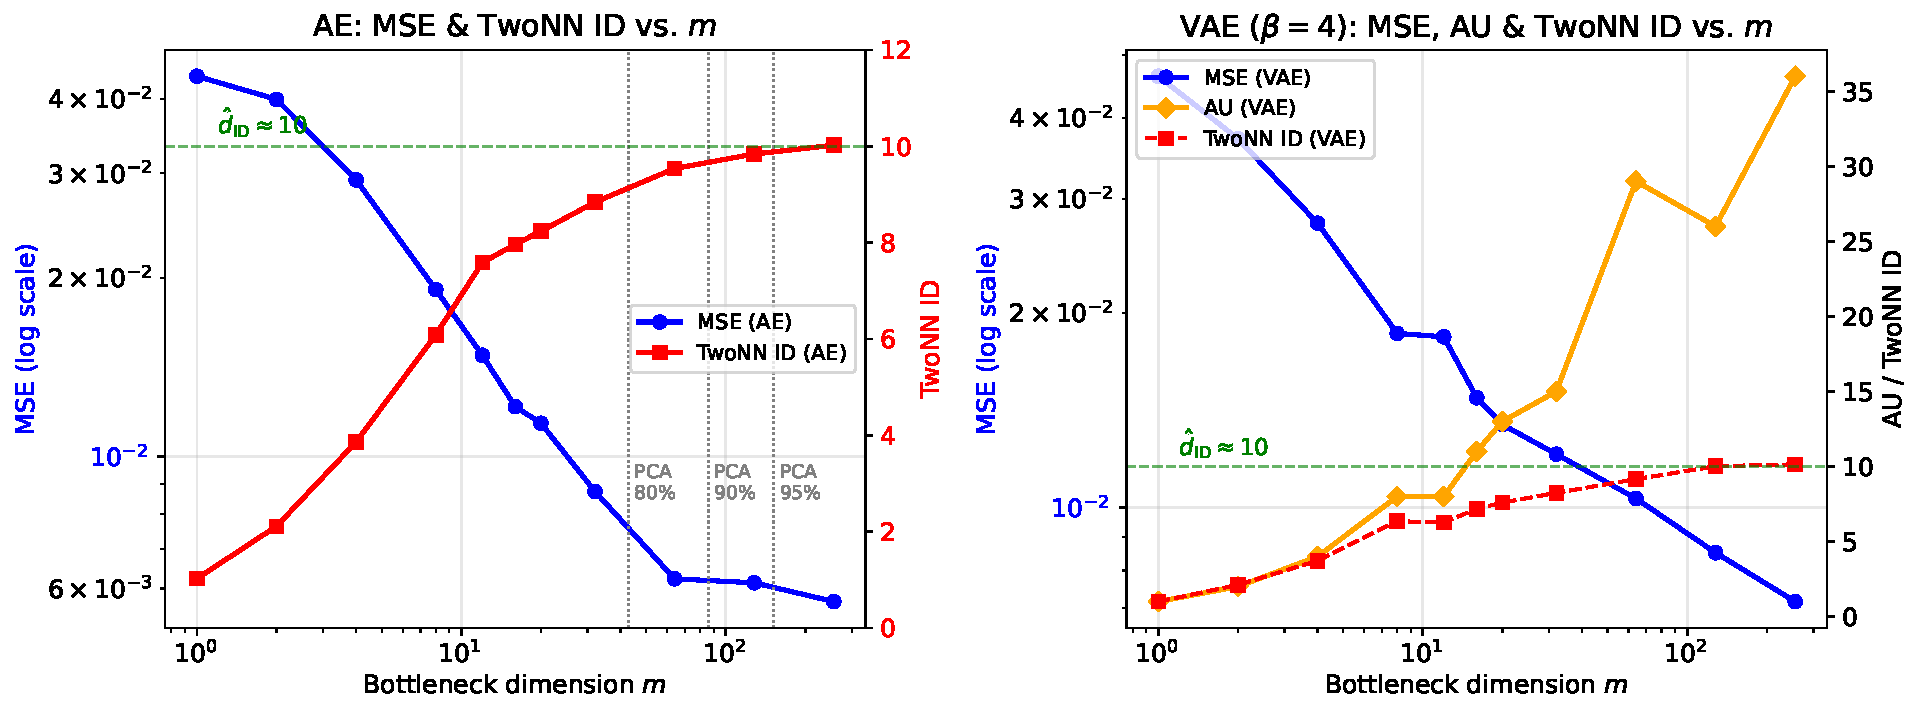
\includegraphics[width=0.95\linewidth]{results/figures/E4_mnist_dualaxis.pdf}
\caption{MNIST: $m$-dependence of the indicators (300 epochs).
\textbf{Left (AE)}: MSE (log scale, left axis) and TwoNN ID (right axis);
vertical dotted lines mark the PCA 80/90/95\% dimensions (43/86/152),
far above the nonlinear estimate $\hatdID \approx 10$.
\textbf{Right (VAE, $\beta = 4$)}: MSE, AU, and TwoNN ID; the AU growth
slows beyond $m \approx \hatdID$.}
\label{fig:e4_dualaxis}
\end{figure}}{}

\IfFileExists{results/figures/E4_300ep_multiseed.pdf}{%
\begin{figure}[H]
\centering
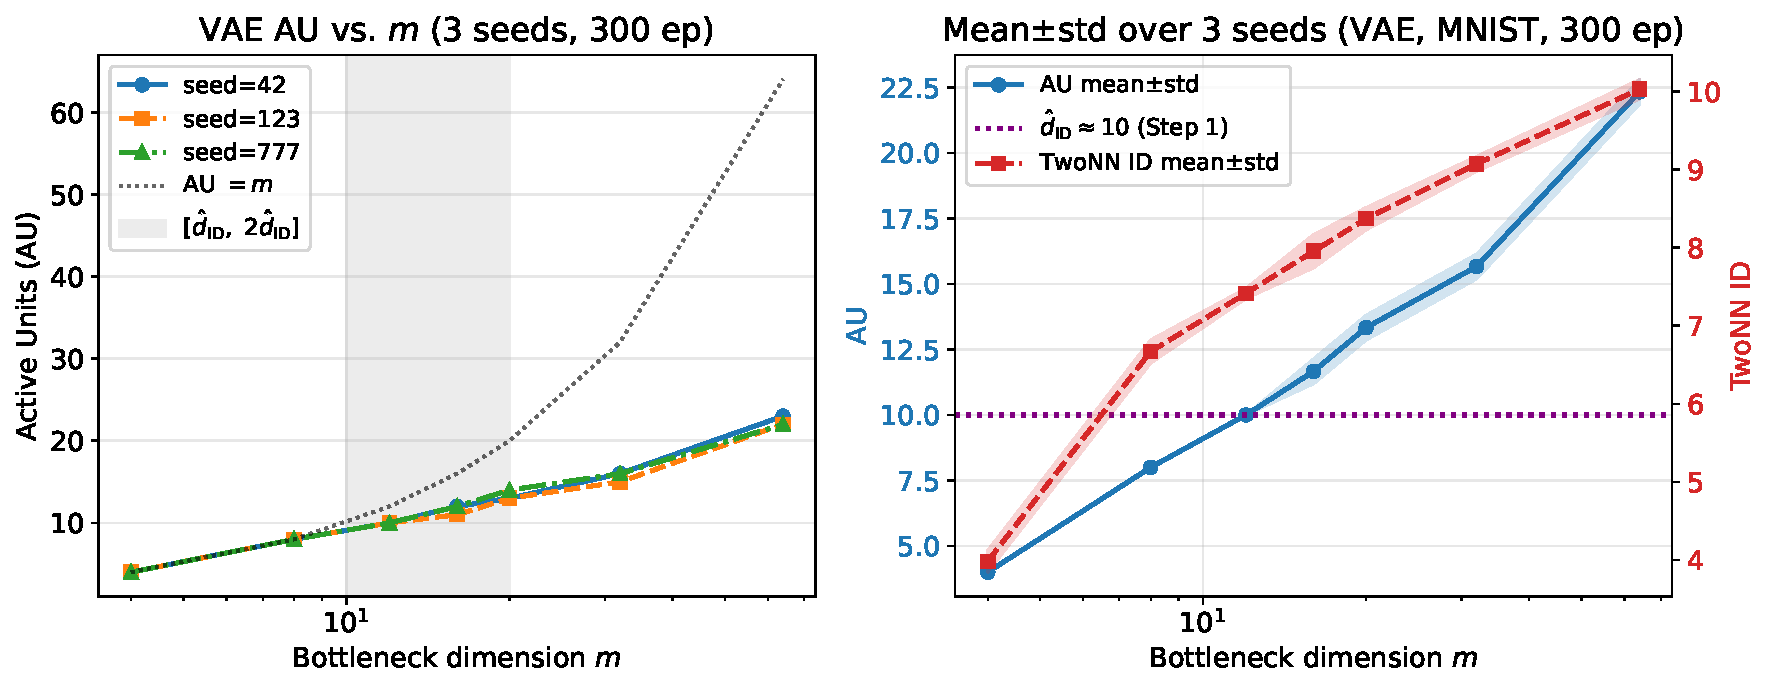
\includegraphics[width=0.9\linewidth]{results/figures/E4_300ep_multiseed.pdf}
\caption{MNIST: multi-seed reproducibility of the AU verification signal
(3 seeds, 300 epochs). Left: per-seed AU$(m)$ with the ID-guided search
window $[\hatdID, 2\hatdID]$ shaded; right: mean$\pm$std band with the Step-1
reference $\hatdID \approx 10$. AU values are highly reproducible
($\sigma \leq 0.5$). Change-point (knee) estimates are deliberately not
shown here; they are exploratory only (Appendix~\ref{app:knee}).}
\label{fig:e4_multiseed}
\end{figure}}{}

\subsubsection{鈍化域の細密観察と変化点検出の注意}\label{sec:exp_mnist_dense}

鈍化の開始位置をより細かく見るため，
$\hatdID$近傍を1刻みにした密グリッド（$m = 8$--$16$を1刻み，
以降$m \in \{18, 20, 24, 28, 32, 40, 48, 64\}$；計17点，300 エポック，3シード）で
AU 曲線を観察した．
AU$(m)$は$m = 8$--10 でほぼ対角（AU $= m$）に乗り，$m \geq 11$で対角から離れ始める——
一階差分比率に基づく変化点検出（閾値$\tau_{\mathrm{knee}} = 0.25$；\ref{app:knee}）を
この密グリッドに適用すると変化点は$10.3 \pm 0.9$（シード別 11, 9, 11）となり，
$\hatdID \approx 10$と整合する．

ただし，この整合には2つの重要な限定がある．
第一に，密グリッド領域は Step 1 の TwoNN 推定値の近傍に置いたものであり，
この結果は\textbf{TwoNN 由来の探索窓に条件付けられた局所的な曲線要約}であって
独立な相互検証ではない．
第二に，同じ検出器を疎グリッド$\{4, 8, 12, 16, 20, 32, 64\}$に適用すると
変化点は$43 \pm 15$と大きく変動する——
\textbf{変化点の自動検出はグリッド設計に強く依存し，
プロトコルの名前付き出力として運用すべきでない}．
このため本プロトコルの Step 3 は「AU 鈍化域が$\hatdID$と同一オーダーにあるか」という
頑健な読み取り（AU 値そのものの多シード比較）を主とし，
変化点検出はグリッド設計の補助にとどめる（詳細な感度分析は\ref{app:knee}）．

\subsubsection{Fashion-MNIST}\label{sec:exp_fashion}

Fashion-MNIST では Exp-Real-Geom（§\ref{sec:exp_real_geom}；3シード，300 エポック）により
$\hatdID \approx 10$を得た：TwoNN は$m_{\mathrm{ref}} = 5d$--$10d$で$9.9$--$10.1$に収束する
（$d = 9$は予備的な 100 エポック推定に基づくスイープのグリッド設計値；\ref{app:exploratory}）．
Step 2 により検証点は$m_{\mathrm{ver}} = 2\hatdID = 20$である．
Step 3 は MNIST と同一プロトコルの3シード検証
（Exp-Fashion-MS；FC-VAE，$\beta = 4$，300 エポック，
$m \in \{4, 8, 12, 16, 20, 32, 64\}$）で行った（表\ref{tab:fashion_s3}）．

結果は，判定規則の診断能力を示す\textbf{境界事例}となった：
AU$(20) = 7.0 \pm 0.0$（3シードで完全一致）であり，
\textbf{V1 は成立}（活性率$0.35 \leq 0.9$；遮断は頑健に機能）する一方，
\textbf{V2 は下側境界で不成立}（AU $= 7 < \hatdID = 10$；シード毎判定も全会一致）である．
表\ref{tab:failure}第3行の診断に従えば，これは
「$\beta = 4$がこのデータ・デコーダの組に対して過正則化側にある」か，
「AE 経由の Step 1 参照値が，この$\beta$のもとで VAE が刈り込む分散方向
（テクスチャ・スタイル的な因子）を含んでいる」ことを示唆する．
実際，MSE の鈍化も$m \approx 12$--16 で生じており（表\ref{tab:fashion_s3}），
AU 鈍化域（7--12）が$\hatdID$と同一オーダーにあるという予備観察
（\ref{app:exploratory}）自体は3シードで再現された．
すなわち Fashion-MNIST は，プロトコルが機械的に合格を返す例ではなく，
\textbf{事前登録した判定規則が実データの境界事例を検出し，
表\ref{tab:failure}の診断へ誘導する}実例である．

\begin{table}[H]
\centering
\caption{Exp-Fashion-MS (Fashion-MNIST FC-VAE, $\beta = 4$, 300 epochs,
mean$\pm$std, 3 seeds). At the pre-specified verification point
$m_{\mathrm{ver}} = 20$, V1 passes (activation ratio $0.35$) while the
lower V2 bound is violated (AU $= 7.0 < \hatdID = 10$) unanimously across
seeds---a diagnostic boundary case (third row of Table~\ref{tab:failure}).}
\label{tab:fashion_s3}
\small
\begin{tabular}{rccc}
\toprule
$m$ & AU & TwoNN ID (latent) & MSE \\
\midrule
 4 & $4.0 \pm 0.0$ & $3.71 \pm 0.10$ & 0.0184 \\
 8 & $6.3 \pm 0.5$ & $5.44 \pm 0.19$ & 0.0152 \\
12 & $7.0 \pm 0.0$ & $5.90 \pm 0.07$ & 0.0144 \\
16 & $7.3 \pm 0.5$ & $6.10 \pm 0.43$ & 0.0141 \\
\textbf{20} & $\boldsymbol{7.0 \pm 0.0}$ & $5.83 \pm 0.17$ & 0.0143 \\
32 & $9.3 \pm 0.5$ & $6.88 \pm 0.22$ & 0.0130 \\
64 & $11.7 \pm 0.5$ & $7.79 \pm 0.06$ & 0.0120 \\
\bottomrule
\end{tabular}
\end{table}

\subsection{ベースライン比較：探索コストと下流性能}\label{sec:exp_downstream}

ID 誘導型選定の実用価値を，
「フル$m$グリッド探索」との比較で定量化する（Exp-Downstream）．
評価指標は潜在表現上の線形プローブ（多クラスロジスティック回帰）による
テスト分類精度と再構成 MSE である．

\textbf{AE（参照 AE スイープの再利用，300 エポック，シード 42）}：
表\ref{tab:downstream}左のとおり，
線形プローブ精度は$m = 8$--12 で頭打ちとなり（$92.3\%$，$m = 12$），
$m = 256$まで増やしても改善しない（$91.8\%$；生ピクセル 784 次元では$91.6\%$）．
\textbf{フルグリッド（11 点）上の最良精度$92.3\%$は
ID 誘導探索窓$[10, 24]$の内部（$m = 12$）で達成され}，
範囲内の他の点（$m = 16, 20$）との差も 1.4 ポイント以内である．

\textbf{VAE（$\beta = 4$，300 エポック，3シード）}：
表\ref{tab:downstream}右のとおり，VAE 側でも同じ構図が成り立つ：
線形プローブ精度はグリッド$\{4, \ldots, 64\}$全体の最良値$89.1 \pm 0.4\%$を
探索窓内の$m = 12$で達成し，$m \geq 12$ではほぼ横ばいである
（VAE 経路の検証点$m = 20 = 2\hatdID$でも$88.2 \pm 0.4\%$と
最良値との差は 1 ポイント未満）．
なお本表の AU・MSE は表\ref{tab:mnist_s3}（Exp-Mnist-Multi-300）の再学習による
再現値であり，両者は一致した（再現性の追加確認）．

\textbf{探索コスト}：本論文の MNIST フルグリッドは$m$ 11 点
$\times$ 3 シード $= 33$ ランを要する．
これに対し ID 誘導経路は，Step 1 の参照 AE（$m_{\mathrm{ref}} \in \{64, 128, 256\}$の
収束確認；単一シードで 3 ラン）ののち，
（a）AE 経路：探索窓$[10, 24]$内のグリッド点$\{12, 16, 20\}$を
3 シードで学習（9 ラン）——計 12 ラン（\textbf{約 64\%削減}）；
（b）VAE 経路：$m = 2\hatdID = 20$の1点を 3 シードで学習し AU で検証（3 ラン）
——計 6 ラン（\textbf{約 82\%削減}），
のいずれでも探索コストを大幅に削減する．
MLE シフト検証点$m = 32$でも併せて検証する保守的な変種
（§\ref{sec:protocol_s3}）では，VAE 経路は計 9 ラン（約 73\%削減）となる．
なおこの会計は Step 1 を単一シードで数えている（本論文の Step 1 は
サブサンプリング CI と推定量相互検証で不確かさを別途定量化しているため）；
Step 1 も 3 シードで行う対称な会計では
AE 経路 18 ラン（約 45\%削減）・VAE 経路 12 ラン（約 64\%削減）となる．
保持される性能は上記のとおり最良値とほぼ同等である．
ただしこの比較は本論文の MNIST グリッド構成・線形プローブに限られ，
一般の削減率を主張するものではない（§\ref{sec:disc_model_selection}）．

\begin{table}[H]
\centering
\caption{Exp-Downstream (MNIST): linear-probe test accuracy and MSE vs.\ $m$.
Left: AE latents (300 epochs, single seed 42; reuse of the reference-AE
sweep). Right: FC-VAE ($\beta = 4$) latents (300 epochs, mean$\pm$std, 3
seeds). Bold $m$ values lie in the ID-guided search window $[10, 24]$,
which contains the best accuracy over the full grid; for the VAE, $m = 20$
is in addition the pre-specified verification point $m_{\mathrm{ver}}$
(§\ref{sec:protocol_s3}).
Raw-pixel baseline: $91.6\%$.}
\label{tab:downstream}
\small
\begin{tabular}{r cc | r ccc}
\toprule
\multicolumn{3}{c|}{AE (single seed)} & \multicolumn{4}{c}{VAE ($\beta = 4$, 3 seeds)} \\
$m$ & Probe acc.\ (\%) & MSE & $m$ & Probe acc.\ (\%) & AU & MSE \\
\midrule
1 & 60.0 & 0.0437 & 4 & $85.0 \pm 0.5$ & $4.0 \pm 0.0$ & 0.0282 \\
2 & 60.0 & 0.0399 & 8 & $87.7 \pm 0.1$ & $8.0 \pm 0.0$ & 0.0182 \\
4 & 81.7 & 0.0292 & \textbf{12} & $\boldsymbol{89.1 \pm 0.4}$ & $10.0 \pm 0.0$ & 0.0154 \\
8 & 91.7 & 0.0191 & \textbf{16} & $89.0 \pm 0.2$ & $11.7 \pm 0.5$ & 0.0138 \\
\textbf{12} & \textbf{92.3} & 0.0148 & \textbf{20} & $88.2 \pm 0.4$ & $13.3 \pm 0.5$ & 0.0126 \\
\textbf{16} & 92.0 & 0.0121 & 32 & $88.1 \pm 0.2$ & $15.7 \pm 0.5$ & 0.0112 \\
\textbf{20} & 90.9 & 0.0114 & 64 & $88.7 \pm 0.3$ & $22.3 \pm 0.5$ & 0.0089 \\
32 & 91.2 & 0.0087 &  & & & \\
64 & 91.8 & 0.0062 &  & & & \\
128 & 92.2 & 0.0061 &  & & & \\
256 & 91.8 & 0.0057 &  & & & \\
\bottomrule
\end{tabular}
\end{table}

\subsection{Step 1 の妥当性条件：何が内在次元推定を安定にするか}\label{sec:exp_real_geom}

Step 1 は参照 AE の潜在表現を経由するため，
「参照表現の幾何的歪みが推定を壊さないか」が焦点となる．
実験 Exp-Real-Geom では，等長性の異なる4モデル
（通常 AE／IsometricAE\cite{kato2020rdae}／CAE\cite{rifai2011cae}／DAE\cite{alain2014dae}）を
MNIST・Fashion-MNIST 上で$m_{\mathrm{ref}} \in \{d, 2d, 3d, 5d, 10d\}$
（$d$は予備推定に基づくグリッド設計値；MNIST は 10，Fashion-MNIST は 9）でスイープし，
TwoNN・MLE・$\kap$・Trustworthiness・kNN overlap を比較した（3シード，300 エポック）．

\begin{table}[H]
\centering
\caption{Exp-Real-Geom (MNIST, mean$\pm$std, 3 seeds): TwoNN through four
reference models. Convergence is driven by the bottleneck margin
$m_{\mathrm{ref}} / \hatdID$, largely independently of the isometry
(condition number $\kap$).}
\label{tab:real_geom}
\small
\begin{tabular}{lcccc}
\toprule
Model & TwoNN ($m_{\mathrm{ref}} = d$) & TwoNN ($m_{\mathrm{ref}} = 5d$) & TwoNN ($m_{\mathrm{ref}} = 10d$) & $\kap$ ($m_{\mathrm{ref}} = 10d$) \\
\midrule
AE          & $7.3 \pm 0.4$ & $10.0 \pm 0.1$ & $10.0 \pm 0.1$ & $4.1 \times 10^{7}$ \\
IsometricAE & $7.5 \pm 0.4$ & $10.1 \pm 0.1$ & $10.1 \pm 0.1$ & $7.8$ \\
CAE         & $7.2 \pm 0.5$ & $9.9 \pm 0.1$  & $10.0 \pm 0.1$ & $3.2 \times 10^{3}$ \\
DAE         & $7.6 \pm 0.4$ & $10.0 \pm 0.1$ & $10.0 \pm 0.1$ & $6.3 \times 10^{3}$ \\
\bottomrule
\end{tabular}
\end{table}

結果（表\ref{tab:real_geom}）は明確である：
（1）4モデルすべてで TwoNN は$m_{\mathrm{ref}} = d$の過小推定（$\approx 7.3$--7.6）から
$m_{\mathrm{ref}} \geq 5d$で$\approx 10$へ収束し，
モデル間差（$\pm 0.3$以内）は$m_{\mathrm{ref}}$増大の効果（約 2.5 ポイント）より
1桁小さい；
（2）IsometricAE は$\kap$を$10^{7}$から$8$前後まで改善するが，
TwoNN への効果は$\pm 0.2$以内にとどまる．
Fashion-MNIST でも同一のパターンを得た．
すなわち\textbf{「等長性の改善」ではなく「ボトルネック余裕$m_{\mathrm{ref}} \gg \hatdID$」が
Step 1 の安定性の支配的条件}であり
（命題\ref{thm:twonn_stability}の$\delta_T$支配の含意と整合），
Step 1 で$m_{\mathrm{ref}} = 256 \gg \hatdID$の通常 AE を使う設計が正当化される
（図\ref{fig:ep}）．

\IfFileExists{results/figures/EP_twonn_stability.pdf}{%
\begin{figure}[H]
\centering
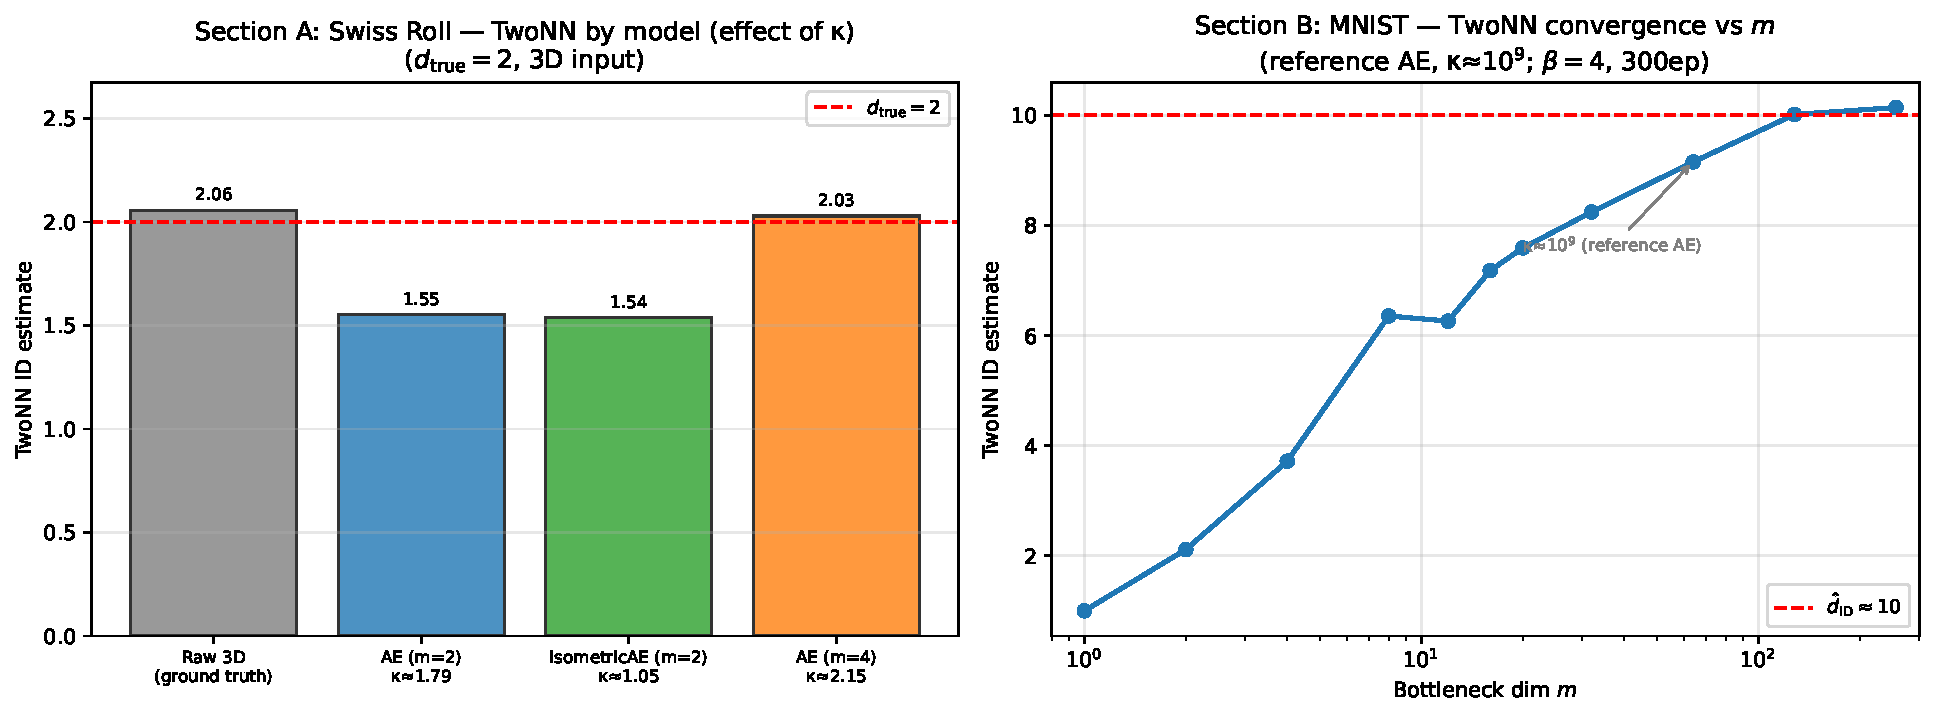
\includegraphics[width=0.95\linewidth]{results/figures/EP_twonn_stability.pdf}
\caption{Step-1 stability: (left) on Swiss Roll, TwoNN recovers once
$m_{\mathrm{ref}} > \dtrue$ regardless of isometry; (right) on MNIST, TwoNN
stabilizes for $m_{\mathrm{ref}} \geq 48 \approx 5\hatdID$ even where the
condition number $\kap$ grows sharply.}
\label{fig:ep}
\end{figure}}{}

\subsection{適用境界：Conv-VAE と自然画像}\label{sec:exp_boundary}

本節はプロトコルの「失敗の報告」ではなく，
表\ref{tab:failure}の失敗モードが実際にどの条件で発生するかの定量化である．

\subsubsection{Conv-VAE：$\beta$不足による遮断の不発（3シード）}

MNIST Conv-VAE（2層 Conv＋2層 ConvTranspose，KL サイクリックアニーリング
$\beta_{\max} = 4$\cite{fu2019cyclical}，150 エポック，3シード）を
$m \in \{4, 8, 16, 32, 64, 96, 128, 192, 256\}$でスイープした（Exp-Conv-M256）．
$m \leq 64$では AU $= m$（遮断なし）が全シードで継続し，
$m = 96$で初めて AU $= 90.7 \pm 1.2 < m$となるが，
$m = 256$でも活性率 94\%と高い（図\ref{fig:en}）．
$m \in \{384, 512\}$への拡張（Exp-Conv-M512）でも AU $\approx m$が維持された——
すなわち$\beta_{\max} = 4$では遮断閾値$\dstar > 512$であり，
\textbf{AU 検証は「$\beta$がデコーダ容量に対して小さすぎる」状態を
AU $= m$という明確な信号で検出する}（表\ref{tab:failure}第1行）．

サロゲート条件（命題\ref{thm:linear_vae}）の観点では，
強力な Conv デコーダは実効ノイズ分散$\tau^2_{\mathrm{eff}}$を小さくし
（FC-VAE の逆算校正値$\approx 0.30$に対し Conv-VAE では$\ll 0.30$；
ヒューリスティックな外挿），閾値$\beta\tau^2_{\mathrm{eff}}$を下げて$\dstar$を膨張させる．
この解釈は$\beta$増強実験と整合する：
$\beta_{\max} = 10$では$m = 256$で AU $= 95.7 \pm 5.2$（活性率 37\%），
$\beta_{\max} = 20$では AU $= 68.0 \pm 2.2$（27\%）と明確な飽和傾向が誘発された
（Exp-ConvV-HiBeta；\textbf{3シード}，詳細は\ref{app:exploratory}）．
$\beta$の増大で遮断が低次元側へ移動するという定性的予測と整合しており，
Conv-VAE でのプロトコル適用には「データ・アーキテクチャに応じた$\beta$の増強」が
必要条件であることが特定された．

\textbf{判定}（MNIST Conv-VAE）：
Step 1——使用可（FC 参照 AE 経由の$\hatdID \approx 10$を流用）；
Step 2——探索窓取得可（$m \geq 20$）；
Step 3——$\beta_{\max} = 4$では\textbf{不合格}（$m = 256$で活性率$0.94 > 0.9$，V1 不成立）．
$\beta_{\max} \in \{10, 20\}$では V1 は成立する
（活性率$0.37$・$0.27$；3シードのシード毎判定でも全会一致）が，
AU $= 95.7 \pm 5.2$・$68.0 \pm 2.2 > 3\hatdID = 30$のため V2 は不成立のままであり，
「遮断は誘発できたが$\hatdID$とのオーダー整合は未達」と判定する．

\IfFileExists{results/figures/EN_conv_vae_extended_m.pdf}{%
\begin{figure}[H]
\centering
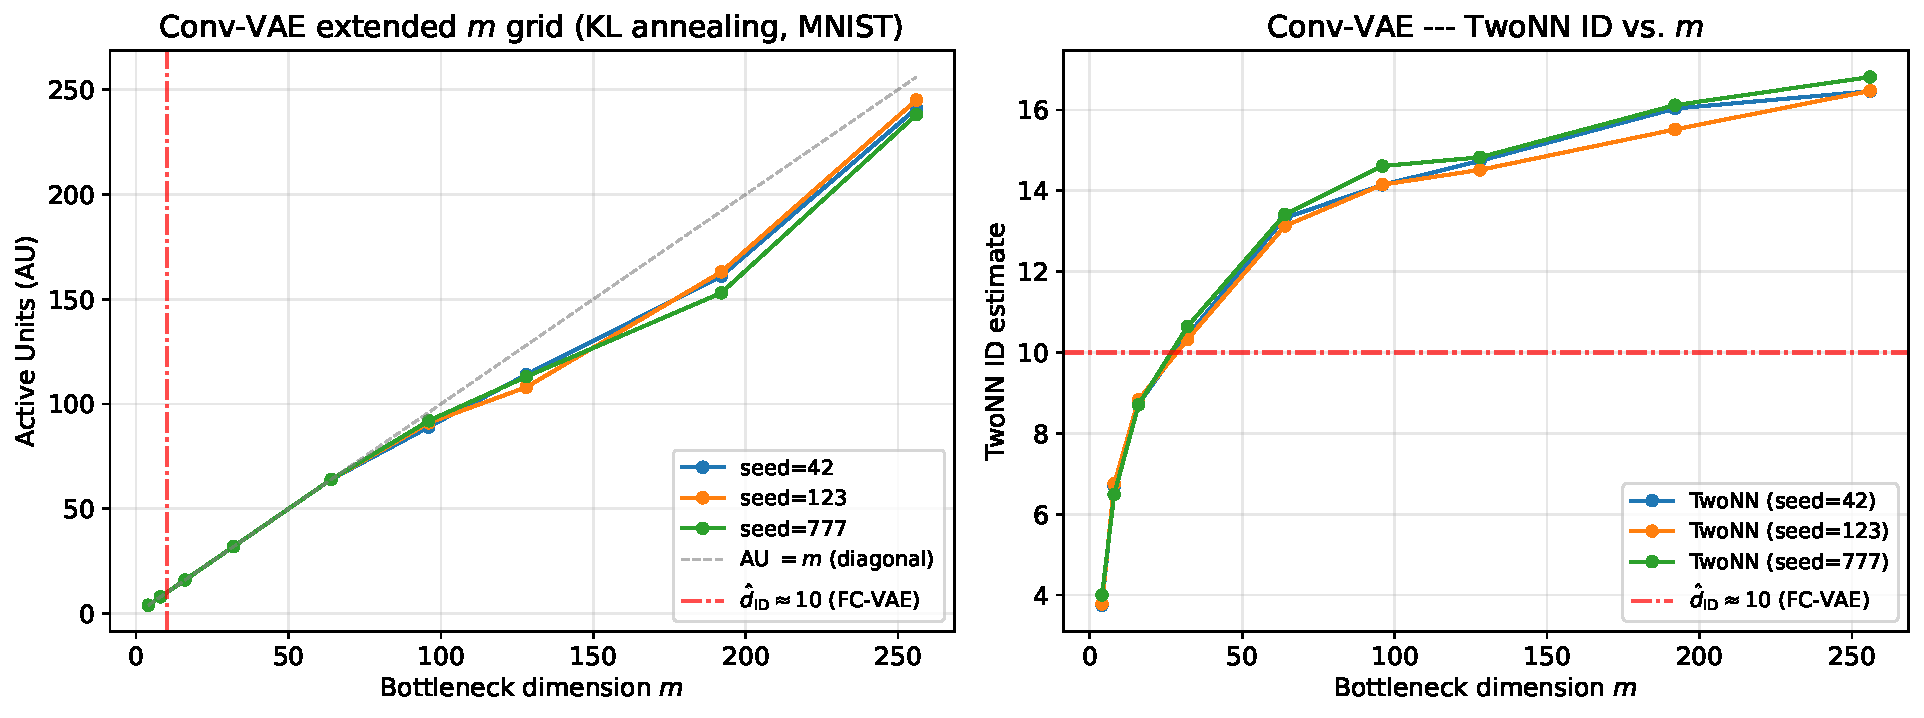
\includegraphics[width=0.95\linewidth]{results/figures/EN_conv_vae_extended_m.pdf}
\caption{Boundary condition (Exp-Conv-M256): MNIST Conv-VAE with
$\beta_{\max} = 4$ keeps AU $= m$ (no truncation) up to $m = 64$ and stays
at 94\% activation even at $m = 256$ --- the failure mode ``$\beta$ too small
relative to decoder power'' detected by the AU signal.}
\label{fig:en}
\end{figure}}{}

\subsubsection{自然画像：Step 1 の有界な信頼域と Step 3 の未達（3シード）}

CIFAR-10\cite{krizhevsky2009learning}・SVHN\cite{netzer2011reading}の
Conv-VAE（3層 Conv，$\beta_{\max} = 4$，150 エポック，3シード，
$m \in \{16, 32, 64, 128, 256\}$）では次の2点が観測された（表\ref{tab:natural}）．
第一に，\textbf{Step 1 は条件付きで機能する}：
CIFAR-10 の潜在 TwoNN は$m = 64 \approx 2\hatdID$で$25.21 \pm 0.41$となり，
生データ推定（25.20）および Pope ら\cite{pope2021intrinsic}の報告値（$\approx 26$）と
整合する．しかし$m \geq 128$では$28.8$--$30.9$へ単調に膨張する——
\textbf{自然画像では$m_{\mathrm{ref}} \approx 2\hatdID$付近でのみ推定が
既報値と整合し，「大きいほど良い」は成り立たない}
（真の内在次元は未知なので「整合」以上は主張できない；
表\ref{tab:failure}第4行の失敗モード）．
MNIST（$m_{\mathrm{ref}} = 25\hatdID$でも安定）との違いは，
AU $= m$のまま全次元が使用され続ける（遮断が効かない）ことによる
潜在幾何の歪みに起因すると解釈される．
SVHN では乖離がさらに大きい（$m = 256$で潜在 27.1 vs.\ 生データ 10.1）．

\textbf{なぜ自然画像で歪みがこれほど顕著になるのか（仮説）}．
MNIST と自然画像の差は程度問題ではなく，データ幾何の質的な違いを反映すると考える．
第一に\textbf{多様体の絡み合い（manifold entanglement）}：
MNIST は中央に正規化された単一物体のストローク変形が主因子であり，
近似的に単一の滑らかな多様体とみなせるのに対し，
自然画像は物体カテゴリ・姿勢・テクスチャ・照明・背景という
スケールの異なる因子の合成であり，
局所次元がクラス・領域ごとに大きく異なる部分多様体の和集合として振る舞う
（Pope ら\cite{pope2021intrinsic}もクラス間で ID が大きく変動することを報告している）．
単一の大域計量を仮定する TwoNN にとって，
このような不均質な構造は$m_{\mathrm{ref}}$の増大とともに
近傍順位の保存（命題\ref{thm:twonn_stability}の$\delta_T$）を悪化させやすい．
第二に\textbf{高周波テクスチャと実効ノイズ分散}：
自然画像の再構成には微細テクスチャの符号化が必要で，
強力な Conv デコーダは$\tau^2_{\mathrm{eff}}$を極端に小さくする．
その結果$\dstar \gg m$となって遮断が消失し，
全座標が使用され続ける潜在空間では
「多様体をなす主要因子＋テクスチャ残差」が同一の計量に混在して
近傍構造が歪む——これは AU $= m$と TwoNN 膨張が
同時に観測されるという本実験のパターンと整合する．
第三に\textbf{階層的潜在構造の必要性}：
大域（物体）から局所（テクスチャ）へのスケール階層をなす生成因子を，
単一のフラットな潜在ベクトルと等方事前分布で表現しようとする
アーキテクチャ上の不整合そのものが歪みの一因である可能性がある．
この仮説のもとでは，階層型 VAE\cite{sonderby2016ladder}の
スケール別潜在にプロトコルを階層ごとに適用する
（各階層の AU を別々に読む）拡張が自然な次の一手となる（§\ref{sec:disc_limitation}）．
いずれの仮説も本実験の観測（AU $= m$の持続・$m_{\mathrm{ref}}$依存の TwoNN 膨張・
$\beta$増強による部分的回復）と整合するが，直接の切り分けは今後の課題である．
第二に，\textbf{Step 3 は未達である}：AU 飽和は$m \leq 256$では現れず
（SVHN で$m \geq 128$から AU $< m$となるのみ），
AU 検証には$\beta$増強・デコーダ容量制限・より大きな$m$域の探索が必要である
（$\beta_{\max} = 80$・薄型デコーダでの plateau-like behavior の予備観察は
\ref{app:exploratory}）．

\textbf{判定}（自然画像）：
Step 1——$m_{\mathrm{ref}} \approx 2\hatdID$の範囲でのみ使用可
（CIFAR-10：$25.21 \pm 0.41$，既報値と整合；それ以上は膨張）；
Step 2——探索窓は条件付きで取得可（CIFAR-10：$m \geq 50$）；
Step 3——\textbf{未解決}（CIFAR-10：$m = 256$で活性率$1.0$，V1 不成立；
SVHN：活性率$0.81$で V1 成立も AU $= 206.7 \gg 3\hatdID$で V2 不成立）．

\begin{table}[H]
\centering
\caption{Natural images (Exp-Nat-Cifar / Exp-Nat-SVHN): Conv-VAE with KL
cyclic annealing ($\beta_{\max} = 4$, 150 epochs, mean$\pm$std, 3 seeds).
For CIFAR-10, Step 1 agrees with Pope et al.~\cite{pope2021intrinsic} only
near $m \approx 2\hatdID$ (for SVHN the latent--raw discrepancy is larger;
see text); Step 3 (AU saturation) is not reached in the tested range.}
\label{tab:natural}
\small
\begin{tabular}{r cc | cc}
\toprule
 & \multicolumn{2}{c|}{CIFAR-10} & \multicolumn{2}{c}{SVHN} \\
$m$ & AU & TwoNN ID & AU & TwoNN ID \\
\midrule
 16 & $16.0 \pm 0.0$ & $13.12 \pm 0.12$ & $16.0 \pm 0.0$ & $11.30 \pm 0.12$ \\
 32 & $32.0 \pm 0.0$ & $19.26 \pm 0.23$ & $32.0 \pm 0.0$ & $15.08 \pm 0.08$ \\
 64 & $64.0 \pm 0.0$ & $\mathbf{25.21 \pm 0.41}$ & $64.0 \pm 0.0$ & $19.97 \pm 0.12$ \\
128 & $128.0 \pm 0.0$ & $28.83 \pm 0.41$ & $125.3 \pm 0.5$ & $24.60 \pm 0.36$ \\
256 & $256.0 \pm 0.0$ & $30.91 \pm 0.64$ & $206.7 \pm 1.2$ & $27.08 \pm 0.34$ \\
\midrule
\multicolumn{3}{l|}{Raw-input TwoNN $= 25.20$, MLE $= 26.56$} &
\multicolumn{2}{l}{Raw-input TwoNN $= 10.09$, MLE $= 18.85$} \\
\bottomrule
\end{tabular}
\end{table}

%% ===================================================================
\section{考察}\label{sec:discussion}

\subsection{従来のモデル選択基準と何が違うか}\label{sec:disc_model_selection}

実務で$m$を選ぶ従来手段は，検証再構成誤差・ELBO の$m$スイープや
下流タスク性能である．これらは「性能が頭打ちになる$m$」を教えるが，
（i）グリッド全域のスイープを要し，
（ii）頭打ちの原因（データの多様体次元か，モデル容量か，最適化か）を区別しない．
本プロトコルはこれらを置き換えるのではなく\textbf{補完}する：
Step 1 がスイープに先立って探索窓を$\hatdID$近傍に絞り込み（探索コストの削減），
Step 3 の AU が「性能とは独立に，何次元が実際に使われているか」を報告することで
冗長次元の有無を直接可視化する．
実際，MNIST では MSE 検証・AU 検証・$\hatdID$・線形プローブ精度の4者が
同一の探索窓$[10, 24]$を支持し（§\ref{sec:exp_downstream}），
探索窓内の$m$の選択は，本論文の MNIST グリッド構成では
フルグリッド探索に対して学習ラン数を約 6〜8 割削減しつつ
下流分類精度をほぼ保持した（一般の削減率を主張するものではない）．
一方，この比較は線形プローブと MNIST に限られ，
非線形の下流タスクや disentanglement 指標との系統比較は今後の課題である．

\subsection{安定性と妥当性：$\hatdID$は何を推定しているか}\label{sec:disc_twonn}

本論文が一貫して維持する区別は，
「TwoNN/MLE が\textbf{数値的に安定}（シード・$m_{\mathrm{ref}}$に対して低分散）」であることと
「\textbf{真の内在次元に対して不偏}」であることは別だ，という点である．
参照 AE の潜在空間は等長でなく（$\kap$は$10^{7}$に達する；表\ref{tab:real_geom}），
TwoNN が推定するのは厳密には「参照表現の局所自由度」である．
MNIST の$\hatdID \approx 10$--12 は，
（i）複数$m_{\mathrm{ref}}$での収束，（ii）TwoNN と MLE の一致，
（iii）モデル4種での一致（表\ref{tab:real_geom}），
（iv）サブサンプリング CI の狭さと原理の異なる推定量（DANCo・ESS）との
オーダー一致（表\ref{tab:boot_ci}），
（v）CIFAR-10 での既報値との整合，という複数の間接証拠に支えられているが，
不偏性の直接証明ではない．
このため本プロトコルは$\hatdID$を「探索窓の中心を与える参照値」として運用し，
Step 3 の検証で閉ループを構成する．
残された課題として，合成データ以外での真値に対する校正
（推定量のバイアス特性の系統評価）を挙げる．

\subsection{AU 検証の限界：変化点検出を名前付き出力にしない理由}\label{sec:disc_knee}

先行版の枠組み（本研究の前身）では AU 鈍化点$\mknee$を診断指標の一つとしていたが，
本論文はこれを名前付き出力から外した．
理由は§\ref{sec:exp_mnist_dense}で示したとおり，
（i）疎グリッドでの検出値（$43 \pm 15$）はグリッド間隔に支配され，
（ii）安定化には TwoNN 由来の探索窓が必要で独立検証にならず，
（iii）検出器（閾値法・二階差分法）の選択にも感度を持つ（\ref{app:knee}）からである．
AU 検証の頑健な部分は「AU 値そのもの（多シードで$\sigma \leq 0.5$）が
$\hatdID$と同一オーダーで鈍化・飽和するか」という読み取りであり，
プロトコルはこの頑健な部分のみを判定規則
（式\eqref{eq:rule_v1}--\eqref{eq:rule_v2}；変化点検出を含まない）に
用いるよう設計した．
探索窓の推定と変化点評価を別シード・別データ部分集合で行う nested validation は
今後の課題である．

\subsection{限界と今後の課題}\label{sec:disc_limitation}

\begin{itemize}
  \item \textbf{検証範囲}：フルプロトコルの多シード検証は合成多様体と
        MNIST・Fashion-MNIST の AU 検証に限られる（MNIST の Step 1 スイープは
        不確かさを別途定量化した単一シード；Fashion-MNIST の Step 3 は
        V1 合格・V2 下側境界違反の診断的検出例；§\ref{sec:exp_fashion}）．
        Conv-VAE の$\beta$増強による遮断の回復（Exp-ConvV-HiBeta）は
        3シードで再現された（V1 成立・V2 未達；§\ref{sec:exp_boundary}）が，
        オーダー整合の達成には$\beta$とデコーダ容量の同時制御が必要である．
  \item \textbf{自然画像での Step 3}：AU 飽和の安定同定は未達であり，
        $\beta_{\max} \in [40, 120]$の密スイープ・デコーダ容量制御・シード安定性の改善が
        今後の課題である（\ref{app:exploratory}）．
        §\ref{sec:exp_boundary}で述べた仮説（多様体の絡み合い・
        テクスチャ起因の$\tau^2_{\mathrm{eff}}$縮小・階層的潜在構造の必要性）は
        改善の方向も示唆する：
        （i）階層型 VAE\cite{sonderby2016ladder}のスケール別潜在に
        プロトコルを階層ごとに適用し，大域因子の階層で AU 遮断を読む；
        （ii）クラス条件付き・領域分割による部分多様体ごとの$\hatdID$推定
        （和集合構造の不均質性の緩和）；
        （iii）デコーダ容量またはレート配分の制御による
        $\tau^2_{\mathrm{eff}}$の下限化（テクスチャ残差を AU 診断から分離する）．
        これらは本プロトコルの枠組み（推定→設定→検証）自体は保ったまま，
        Step 1 と Step 3 を階層・部分集合単位に細分化する拡張である．
  \item \textbf{$\beta$依存性と判定閾値}：AU 検証の読み取りは$\beta$に依存する
        （$\beta \in [2, 8]$で AU パターンの安定性を確認済み；\ref{app:sens}）．
        $\dstar$の$\beta$依存性を積極的に利用した「$\beta$スイープによる
        スペクトル読み取り」は興味深い拡張である．
        また判定規則の閾値（活性率$0.9$・係数$3$）は本論文の設定で
        合格・不合格を大きなマージンで分離する作業既定値であり，
        より多様なデータでの校正は今後の課題である．
  \item \textbf{理論の射程}：命題\ref{thm:linear_vae}は線形ガウス近似であり，
        非線形への外挿は$\tau^2_{\mathrm{eff}}$による事後的な整合確認にとどまる．
        非線形設定での活性化条件の導出は未解決である．
  \item \textbf{計算コスト}：Step 3 の多シード$m$スイープは GPU 時間で数時間〜1日規模を要する．
        Step 1 による候補絞り込みでスイープ域は縮小するが，
        さらなる軽量化（早期エポックでの AU 予測等）は今後の課題である．
\end{itemize}

%% ===================================================================
\section{むすび}\label{sec:conclusion}

本論文は，「AE/VAE のボトルネック次元$m$は入力データの多様体次元から決められるか」
という問いに対し，
\textbf{条件付き・診断型の ID 誘導プロトコル}——
（S1）$m_{\mathrm{ref}} \gg \hatdID$の参照表現による内在次元推定，
（S2）$\hatdID$に位相的余裕を加えた$m$の設定
（AE：$m \in [\hatdID, 2\hatdID]$，VAE：$m \geq 2\hatdID$），
（S3）合否判定規則 V1/V2 を備えた AU・MSE による学習後検証——という回答を与えた．
主張は一般解ではなく次の条件付きの形をとる：
\textbf{$\hatdID$は探索窓を与え，適切な$\beta$とアーキテクチャのもとで
AU が「VAE が余剰次元を実際に遮断したか」を診断する}．
理論面では位相的下界と水充填型サロゲート活性化条件$\lambda_j > \beta\tau^2$が
各ステップの理論的根拠（rationale）を与え，
実験面では真の次元既知の合成多様体
（十分な余裕——Torus では$m \geq 5$——のもとで$\AUsat = \dtrue$または$\demb$；
境界域$m \leq 4$の過剰刈り込みは MSE 検証が検出；3--5シード，$\sigma = 0$）と
MNIST の全結合 VAE（$\hatdID = 10.03 \pm 0.12$と AU 鈍化域の整合；3シード）で
フルプロトコルが判定規則のもとで機能し
（Fashion-MNIST の3シード検証では判定規則が V1 合格・V2 下側境界違反という
過剰刈り込み側の境界事例を診断的に検出），
ID 誘導範囲が本論文の MNIST グリッド構成で
フルグリッド探索の学習ランを約 6〜8 割削減しつつ
下流分類精度を保持することを確認した．
同時に，適用境界を定量化した：
内在次元推定はボトルネック余裕$m_{\mathrm{ref}} \gg \hatdID$でのみ安定であり
（等長性改善は副次的；4モデル比較），
自然画像では$m_{\mathrm{ref}} \approx 2\hatdID$を超えると膨張する；
Conv-VAE では$\beta$不足が AU $= m$（V1 不成立）として検出され，
$\beta$増強で遮断は回復するが$\hatdID$とのオーダー整合（V2）は未達である
（3シード）．
今後の主要課題は，自然画像・Conv-VAE での Step 3 の多シード安定同定，
変化点検出の nested validation，および$\hatdID$のバイアス校正である．

%% ===================================================================
\begin{thebibliography}{99}

\bibitem{kingma2014vae}
D.~P. Kingma and M.~Welling,
``Auto-encoding variational Bayes,''
in \textit{Proc.\ Int.\ Conf.\ Learning Representations (ICLR)}, 2014.

\bibitem{bengio2013representation}
Y.~Bengio, A.~Courville, and P.~Vincent,
``Representation learning: A review and new perspectives,''
\textit{IEEE Trans.\ Pattern Anal.\ Mach.\ Intell.}, vol.~35, no.~8,
pp.~1798--1828, 2013.

\bibitem{lucas2019elbo}
J.~Lucas, G.~Tucker, R.~B. Grosse, and M.~Norouzi,
``Don't blame the ELBO! A linear VAE perspective on posterior collapse,''
in \textit{Advances in Neural Information Processing Systems (NeurIPS)},
vol.~32, 2019.

\bibitem{fefferman2016manifold}
C.~Fefferman, S.~Mitter, and H.~Narayanan,
``Testing the manifold hypothesis,''
\textit{J.\ Amer.\ Math.\ Soc.}, vol.~29, no.~4, pp.~983--1049, 2016.

\bibitem{facco2017twonn}
E.~Facco, M.~d'Errico, A.~Rodriguez, and A.~Laio,
``Estimating the intrinsic dimension of datasets by a minimal neighborhood
information,''
\textit{Sci.\ Rep.}, vol.~7, 12140, 2017.

\bibitem{pope2021intrinsic}
P.~Pope, C.~Zhu, A.~Abdelkader, M.~Goldblum, and T.~Goldstein,
``The intrinsic dimension of images and its impact on learning,''
in \textit{Proc.\ Int.\ Conf.\ Learning Representations (ICLR)}, 2021.

\bibitem{ansuini2019intrinsic}
A.~Ansuini, A.~Laio, J.~H. Macke, and D.~Zoccolan,
``Intrinsic dimension of data representations in deep neural networks,''
in \textit{Advances in Neural Information Processing Systems (NeurIPS)},
vol.~32, 2019.

\bibitem{valeriani2023geometry}
L.~Valeriani, D.~Doimo, F.~Cuturello, A.~Laio, A.~Ansuini, and A.~Cazzaniga,
``The geometry of hidden representations of large transformer models,''
in \textit{Advances in Neural Information Processing Systems (NeurIPS)},
vol.~36, 2023.

\bibitem{higgins2017betavae}
I.~Higgins, L.~Matthey, A.~Pal, C.~Burgess, X.~Glorot, M.~Botvinick,
S.~Mohamed, and A.~Lerchner,
``$\beta$-VAE: Learning basic visual concepts with a constrained variational
framework,''
in \textit{Proc.\ Int.\ Conf.\ Learning Representations (ICLR)}, 2017.

\bibitem{alain2014dae}
G.~Alain and Y.~Bengio,
``What regularized auto-encoders learn from the data-generating
distribution,''
\textit{J.\ Mach.\ Learn.\ Res.}, vol.~15, pp.~3743--3773, 2014.

\bibitem{rifai2011cae}
S.~Rifai, P.~Vincent, X.~Muller, X.~Glorot, and Y.~Bengio,
``Contractive auto-encoders: Explicit invariance during feature extraction,''
in \textit{Proc.\ Int.\ Conf.\ Machine Learning (ICML)}, 2011.

\bibitem{birdal2021intrinsic}
T.~Birdal, A.~Lou, L.~J. Guibas, and U.~Simsekli,
``Intrinsic dimension, persistent homology and generalization in neural
networks,''
in \textit{Advances in Neural Information Processing Systems (NeurIPS)},
vol.~34, 2021.

\bibitem{levina2005mle}
E.~Levina and P.~J. Bickel,
``Maximum likelihood estimation of intrinsic dimension,''
in \textit{Advances in Neural Information Processing Systems (NeurIPS)},
vol.~17, 2005.

\bibitem{ceruti2014danco}
C.~Ceruti, S.~Bassis, A.~Rozza, G.~Lombardi, E.~Casiraghi, and
P.~Campadelli,
``DANCo: An intrinsic dimensionality estimator exploiting angle and norm
concentration,''
\textit{Pattern Recognit.}, vol.~47, no.~8, pp.~2569--2581, 2014.

\bibitem{tippingbishop1999ppca}
M.~E. Tipping and C.~M. Bishop,
``Probabilistic principal component analysis,''
\textit{J.\ Roy.\ Statist.\ Soc.\ Ser.\ B}, vol.~61, no.~3, pp.~611--622,
1999.

\bibitem{bishop1999bayesian}
C.~M. Bishop,
``Bayesian PCA,''
in \textit{Advances in Neural Information Processing Systems (NeurIPS)},
vol.~11, pp.~382--388, 1999.

\bibitem{ghahramani2005infinite}
Z.~Ghahramani and T.~L. Griffiths,
``Infinite latent feature models and the Indian buffet process,''
in \textit{Advances in Neural Information Processing Systems (NeurIPS)},
vol.~18, 2005.

\bibitem{nazari2023geometric}
P.~Nazari, S.~Damrich, and F.~A. Hamprecht,
``Geometric autoencoders---what you see is what you decode,''
in \textit{Proc.\ Int.\ Conf.\ Machine Learning (ICML)}, PMLR vol.~202, 2023.

\bibitem{kato2020rdae}
K.~Kato, J.~Zhou, T.~Sasaki, and A.~Nakagawa,
``Rate-distortion optimization guided autoencoder for isometric embedding in
Euclidean latent space,''
in \textit{Proc.\ Int.\ Conf.\ Machine Learning (ICML)}, PMLR vol.~119, 2020.

\bibitem{hatcher2002algebraic}
A.~Hatcher,
\textit{Algebraic Topology}.
Cambridge, UK: Cambridge University Press, 2002.

\bibitem{lecun1998}
Y.~LeCun, L.~Bottou, Y.~Bengio, and P.~Haffner,
``Gradient-based learning applied to document recognition,''
\textit{Proc.\ IEEE}, vol.~86, no.~11, pp.~2278--2324, 1998.

\bibitem{xiao2017fashion}
H.~Xiao, K.~Rasul, and R.~Vollgraf,
``Fashion-MNIST: A novel image dataset for benchmarking machine learning
algorithms,''
\textit{arXiv preprint} arXiv:1708.07747, 2017.

\bibitem{kornblith2019cka}
S.~Kornblith, M.~Norouzi, H.~Lee, and G.~Hinton,
``Similarity of neural network representations revisited,''
in \textit{Proc.\ Int.\ Conf.\ Machine Learning (ICML)}, PMLR vol.~97,
pp.~3519--3529, 2019.

\bibitem{johnsson2015ess}
K.~Johnsson, C.~Soneson, and M.~Fontes,
``Low bias local intrinsic dimension estimation from expected simplex
skewness,''
\textit{IEEE Trans.\ Pattern Anal.\ Mach.\ Intell.}, vol.~37, no.~1,
pp.~196--202, 2015.

\bibitem{fu2019cyclical}
H.~Fu, C.~Tan, B.~Peng, Z.~Zhao, T.~Yan, C.~Chang, and L.~Zhao,
``Cyclical annealing schedule: A simple approach to mitigating KL
vanishing,''
in \textit{Proc.\ NAACL-HLT}, pp.~240--250, 2019.

\bibitem{krizhevsky2009learning}
A.~Krizhevsky,
``Learning multiple layers of features from tiny images,''
Technical Report, University of Toronto, 2009.

\bibitem{netzer2011reading}
Y.~Netzer, T.~Wang, A.~Coates, A.~Bissacco, B.~Wu, and A.~Y. Ng,
``Reading digits in natural images with unsupervised feature learning,''
in \textit{NIPS Workshop on Deep Learning and Unsupervised Feature
Learning}, 2011.

\bibitem{sonderby2016ladder}
C.~K. S{\o}nderby, T.~Raiko, L.~Maal{\o}e, S.~K. S{\o}nderby, and O.~Winther,
``Ladder variational autoencoders,''
in \textit{Advances in Neural Information Processing Systems (NeurIPS)},
vol.~29, 2016.

\bibitem{cover2006elements}
T.~M. Cover and J.~A. Thomas,
\textit{Elements of Information Theory}, 2nd~ed.
Hoboken, NJ: Wiley-Interscience, 2006.

\bibitem{hoffman2016elbo}
M.~D. Hoffman and M.~J. Johnson,
``ELBO surgery: Yet another way to carve up the variational evidence lower
bound,''
in \textit{NIPS Workshop on Advances in Approximate Bayesian Inference},
2016.

\end{thebibliography}

%% ===================================================================
\appendix

\section{証明と導出}\label{app:proofs}

\subsection{命題\ref{thm:linear_vae}（サロゲート活性化条件）の導出スケッチ}

線形エンコーダ$f(x) = W_e x$，線形デコーダ$g(z) = W_d z$，
事前分布$p(z) = \mathcal{N}(0, I_m)$，
尤度$p(x|z) = \mathcal{N}(W_d z, \tau^2 I_N)$の$\beta$-VAE を考える．
入力を PCA 基底に取り，共分散を$\Sigma = \mathrm{diag}(\lambda_1, \ldots, \lambda_N)$
（$\lambda_1 \geq \lambda_2 \geq \cdots$）とすると，
線形ガウスモデルでは$\beta$-ELBO が固有方向ごとに分離する．
第$j$方向に割り当てるレート（KL 寄与）を$R_j \geq 0$，
そのときの歪み低減を$D_j(R_j)$とすると，ガウス rate--distortion 関数より
$D_j(R_j) = \lambda_j e^{-2R_j}$（nats）であり，$\beta$-ELBO の該当項は
\begin{equation}
  \mathcal{L}_j(R_j) = -\frac{1}{2\tau^2}\lambda_j e^{-2R_j} - \beta R_j + \text{const.}
\end{equation}
$R_j$についての最適化は凹計画であり，KKT 条件
$\partial \mathcal{L}_j / \partial R_j = 0$から
$R_j^* = \max\bigl(0, \tfrac{1}{2}\log(\lambda_j / \beta\tau^2)\bigr)$を得る．
$R_j^* > 0 \iff \lambda_j > \beta\tau^2$が活性化条件（式\eqref{eq:au_threshold}）である．
これは Shannon の水充填定理\cite{cover2006elements}の「水面」を$\beta\tau^2$とした形に一致し，
$\beta = 1$では PPCA\cite{tippingbishop1999ppca}の既知の結果に帰着する．
$m$本の座標が使えるとき，最適解は上位$\min(m, \dstar)$方向を活性化するので
主張（2）（3）が従う．

\textbf{近似の内容}：この導出は，VAE の期待 KL 項
$\mathbb{E}_x[\mathrm{KL}(q_\phi(z|x)\,\|\,p(z))]$を
相互情報量$I(x; z)$（レート）で置き換えている．
両者の差は，いわゆる ELBO surgery 分解\cite{hoffman2016elbo}
\begin{equation}
  \mathbb{E}_x[\mathrm{KL}(q_\phi(z|x)\,\|\,p(z))]
  = I(x; z) + \mathrm{KL}(q_\phi(z)\,\|\,p(z))
  \label{eq:elbo_surgery}
\end{equation}
における aggregated posterior $q_\phi(z)$と事前分布$p(z)$の不一致
$\mathrm{KL}(q_\phi(z)\,\|\,p(z)) \geq 0$であり，
この項を無視できる範囲でのみ本命題は成立する．

\textbf{不一致項の挙動（非線形最適化への含意）}：
落とした不一致項がどう振る舞うかを整理しておく．
（i）線形ガウス設定では，この近似は大域最適解において厳密である：
水充填解の各活性座標では事後平均の周辺分散と事後分散の和が事前分散に一致し
（pPCA 型最適解の性質\cite{tippingbishop1999ppca,lucas2019elbo}），
遮断座標では$q_\phi(z_j|x) = p(z_j)$なので，
$q_\phi(z)$は$p(z)$に一致して$\mathrm{KL}(q_\phi(z)\,\|\,p(z)) = 0$となる．
（ii）非線形 VAE の学習中はこの項は一般に正であり，
学習初期（事後分布が事前分布に近い段階）には小さく，
座標が活性化して aggregated posterior がクラスタ構造
（マルチモーダル性）を獲得するにつれ増大しうる．
（iii）式\eqref{eq:elbo_surgery}より，不一致項が大きいほど
同じ相互情報量（レート）に対して実際の KL ペナルティは大きくなる——
すなわち非線形設定では$\beta$が実効的に増幅されて働き，
本命題の閾値$\lambda_j > \beta\tau^2$による予測は
\textbf{遮断を過小評価する側（活性次元数を過大に見積もる側）}にずれる．
この向きの整理は本論文の使い方と整合する：
Conv-VAE・自然画像で観測された「遮断の不発」（AU $= m$；§\ref{sec:exp_boundary}）は
不一致項では説明できず（不一致項は遮断を強める向きにしか働かない），
デコーダ容量による$\tau^2_{\mathrm{eff}}$の縮小という別機構を要請する——
これが§\ref{sec:exp_boundary}の解釈の根拠である．
逆に，MNIST で AU が$\hatdID$よりやや大きい水準で緩やかに鈍化する観察（§\ref{sec:exp_mnist}）は，
クラスタ構造による不一致項の増大が遮断を保守側へ押す効果と定性的に矛盾しない．
学習中の$\mathrm{KL}(q_\phi(z)\,\|\,p(z))$の系統的測定による
この読みの直接検証は今後の課題である．
また学習された非線形 VAE の勾配ダイナミクスは扱っておらず，
本命題の非線形設定への含意はあくまで定性的である．

\subsection{命題\ref{thm:twonn_stability}（TwoNN 条件付き安定性）の証明スケッチ}

bi-Lipschitz 条件より各距離の変化率は$(1 \mp \varepsilon)^2$の範囲に収まる．
TwoNN 統計量$r_2/r_1$は距離の比であるため一様スケーリングはキャンセルされ，
非等長成分（$\varepsilon \neq 0$）のみが比を歪める．
Trustworthiness $\geq 1 - \delta_T$は 2 近傍の順位保存を高確率で保証し，
順位逆転による$r_2/r_1$の大変動を確率的に抑える．
両条件下で$r_2/r_1$の経験分布の変化（EMD）は連続関数$C(\varepsilon, \delta_T)$で上界され，
TwoNN 推定値のずれもこれに支配される
（$\varepsilon = \delta_T = 0$で$C = 0$）．
有限サンプル・有限次元での近似であり，厳密な定数は設定に依存する．

\subsection{その他の解釈的命題}

\textbf{プルバック計量と局所等長性}：
デコーダ$g$が局所等長であるための必要十分条件は
$G(z) = \Jg(z)^\top \Jg(z) = I_m$である．
条件数$\kap = \sigma_{\max}(\Jg)/\sigma_{\min}(\Jg)$は異方性の指標であり，
$\kap = 1$は等方性のみを意味し等長性までは保証しない．
また$\kap$は局所的な計量診断であって，TwoNN を左右する近傍順位の歪みを
完全には特徴づけない．本論文の$\kap$は歪みの補助指標として用いる．

\textbf{デコーダヤコビアンの実効階数}：
十分な容量の AE が多様体$\mathcal{M}$を正確に再構成するとき，
$\Jg(z)$の有意特異値数は$\min(m, \demb)$に一致する
（有限容量・最適化誤差は無視した理想化）．

\section{AU 変化点検出の探索的解析}\label{app:knee}

本付録は，AU 曲線上の変化点（knee）$\mknee$の自動検出を
名前付きプロトコル出力とし\textbf{ない}判断（§\ref{sec:disc_knee}）の根拠となる
感度データをまとめる．

\subsection{定義}

グリッド$\mathcal{M} = \{m_1 < \cdots < m_K\}$上の AU 増加率を
$s(m_i) = [\mathrm{AU}(m_i) - \mathrm{AU}(m_{i-1})] / (m_i - m_{i-1})$，
正規化増加率を$\rho(m_i) = s(m_i) / \max_j s(m_j)$とし，
\begin{equation}
  \mknee = \min\{m_i \in \mathcal{M} : \rho(m_i) < \tau_{\mathrm{knee}}\},
  \quad \tau_{\mathrm{knee}} = 0.25
  \label{eq:mknee}
\end{equation}
と定義する（一階差分比率法）．
代替として AU$(m)$の離散二階差分の絶対値最大点を取る二階差分法（d2 法）がある．

\subsection{グリッド感度}

理想化された単調飽和モデル（AU が$\dstar$で段差的に飽和し，ノイズなし）では
$|\mknee(\mathcal{M}) - \dstar| \leq \max_i (m_{i+1} - m_i)$が成り立つ
（検出誤差はグリッド最大間隔で上界される）．
実際の MNIST FC-VAE（$\beta = 4$，300 エポック，3シード）では
経験的 AU 曲線の確率的揺らぎによりこの上界を超える変動が生じる（表\ref{tab:knee_grid}）．

\begin{table}[H]
\centering
\caption{Grid sensitivity of the change-point detector on MNIST FC-VAE
($\tau_{\mathrm{knee}} = 0.25$, 3 seeds). The sparse-grid value is dominated
by the grid interval; the dense grid is placed around the TwoNN estimate and
is therefore a TwoNN-conditioned curve summary, not independent validation.}
\label{tab:knee_grid}
\small
\begin{tabular}{lccccc}
\toprule
Condition & Max.\ interval & seed 42 & seed 123 & seed 777 & Mean$\pm$std \\
\midrule
Sparse grid, 150 ep & 32 & 64 & 32 & 64 & $53 \pm 15$ \\
Sparse grid, 300 ep & 32 & 64 & 32 & 32 & $43 \pm 15$ \\
Dense grid, 300 ep & 16 (step 1 in 8--16) & 11 & 9 & 11 & $10.3 \pm 0.9$ \\
\bottomrule
\end{tabular}
\end{table}

エポック延長（150→300）はほとんど効かず，主因は収束不足ではなく
グリッド設計とシードである．
また，単一シード・別グリッドの予備観察では$\mknee = 12$も観測されており
（Exp-Mnist-Base），グリッド・初期化への依存が明確である．

\subsection{検出法・閾値の感度}

密グリッドデータに対する$\tau$法と d2 法の比較を表\ref{tab:knee_method}に示す．
d2 法は遷移域の AU 揺らぎ（8→10→9→11→10→11→13 等）に敏感で，
シード 123 で$\mknee = 28$と大きく外れた．
$\tau_{\mathrm{knee}} = 0.25$は本研究の作業的既定値であり，
Fashion-MNIST では$\tau$の境界感度（$\tau$前後で検出値が変わる）が確認されている——
$\tau_{\mathrm{knee}}$に一般的な意味は主張しない．

\begin{table}[H]
\centering
\caption{Detector sensitivity on the dense grid (300 ep, 3 seeds).}
\label{tab:knee_method}
\small
\begin{tabular}{lcccc}
\toprule
Method & seed 42 & seed 123 & seed 777 & Mean$\pm$std \\
\midrule
$\tau$-method ($\tau = 0.25$) & 11 & 9 & 11 & $10.3 \pm 0.9$ \\
Second difference (d2) & 15 & 28 & 12 & $18.3 \pm 6.8$ \\
\midrule
\multicolumn{5}{l}{Reference: $\hatdID \approx 10$ (TwoNN, 3-seed mean)} \\
\bottomrule
\end{tabular}
\end{table}

\subsection{結論}

変化点検出はグリッド・シード・検出器・閾値のすべてに感度を持ち，
安定化には TwoNN 由来の探索窓という循環的条件が必要である．
したがって本プロトコルでは，変化点はグリッド設計の補助
（$\hatdID$近傍を密にサンプリングする位置の目安）にとどめ，
検証の判定は AU 値そのものの多シード比較で行う．
探索窓推定と変化点評価を分離した nested validation は今後の課題である．

\section{探索的・境界実験の詳細}\label{app:exploratory}

本付録のうち Exp-ConvV-HiBeta は\textbf{3シード（42, 123, 777）の境界実験}であり
本文§\ref{sec:exp_boundary}の判定の根拠となる；
それ以外は\textbf{単一シード（42）または部分的な探索的観察}であり，
本文の主張の直接の根拠には用いていない．

\subsection{Conv-VAE の高$\beta$誘発実験（Exp-ConvV-HiBeta）}

MNIST Conv-VAE（KL サイクリックアニーリング，150 エポック，
$m \in \{16, 32, 64, 96, 128, 192, 256\}$，3シード）で
$\beta_{\max}$を増強した結果を表\ref{tab:hibeta}に示す（Exp-ConvV-HiBeta-MS）．
$\beta_{\max} = 10$で活性率が$m = 256$において 37\%まで低下し，
$\beta_{\max} = 20$ではさらに低次元側へ移動する．
挙動は3シードで一貫しており（$m = 256$のシード間標準偏差は AU で 5 前後），
$\beta$増大で遮断が低次元側へ移動するというサロゲート条件の定性的予測と整合する
（図\ref{fig:hibeta}）．

\begin{table}[H]
\centering
\caption{Exp-ConvV-HiBeta (mean$\pm$std, 3 seeds): AU of the MNIST
Conv-VAE under strengthened $\beta_{\max}$ (mean activation rate in
parentheses). The $\beta_{\max} = 4$ column is the 3-seed Exp-Conv-M256
reference.}
\label{tab:hibeta}
\small
\begin{tabular}{rccc}
\toprule
$m$ & $\beta_{\max} = 4$ & $\beta_{\max} = 10$ & $\beta_{\max} = 20$ \\
\midrule
 32 & $32.0 \pm 0.0$ (100\%) & $32.0 \pm 0.0$ (100\%) & $26.7 \pm 0.5$ (83\%) \\
 64 & $64.0 \pm 0.0$ (100\%) & $52.3 \pm 3.1$ (82\%) & $39.3 \pm 2.5$ (61\%) \\
128 & $111.7 \pm 2.6$ (87\%) & $72.3 \pm 2.5$ (57\%) & $52.7 \pm 0.5$ (41\%) \\
256 & $241.3 \pm 2.9$ (94\%) & $95.7 \pm 5.2$ (37\%) & $68.0 \pm 2.2$ (27\%) \\
\bottomrule
\end{tabular}
\end{table}

\IfFileExists{results/figures/Exp_ConvV_HiBeta.pdf}{%
\begin{figure}[H]
\centering
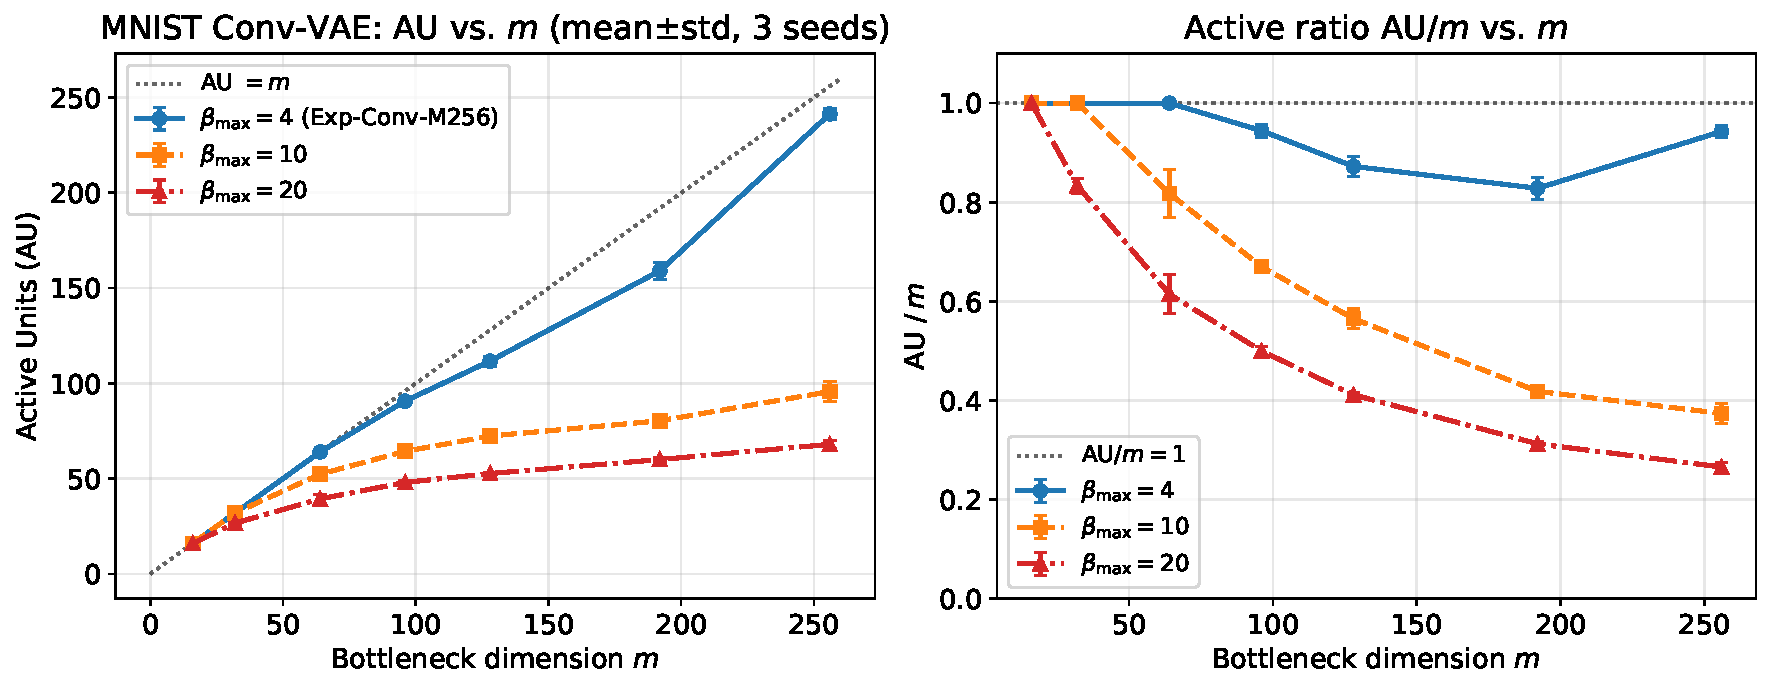
\includegraphics[width=0.9\linewidth]{results/figures/Exp_ConvV_HiBeta.pdf}
\caption{Exp-ConvV-HiBeta (mean$\pm$std, 3 seeds): increasing
$\beta_{\max}$ shifts the AU truncation to lower dimensions, consistent with
the surrogate activation condition.}
\label{fig:hibeta}
\end{figure}}{}

\subsection{自然画像での AU プラトー探索（Exp-NatImg-Sweep）}

CIFAR-10 Conv-VAE で$m \in [32, 1024]$，$\beta_{\max} \in \{10, 20, 40, 80\}$，
デコーダ容量（Standard/Deep/Thin）を組み合わせたスイープでは，
$\beta_{\max} = 80$・薄型デコーダ条件で$m \in [512, 1024]$にわたり
AU $\approx 24$付近の plateau-like behavior が観測された（予備的証拠）．
全条件で潜在 TwoNN は$24.7$--$25.4$と安定し，
Pope ら\cite{pope2021intrinsic}の報告値と整合した．
シード安定性・グリッド安定性を含む安定同定は未達であり，今後の課題である．

\subsection{Fashion-MNIST の VAE 予備観察（Exp-Fashion）}

本文§\ref{sec:exp_fashion}の3シード検証（Exp-Fashion-MS）に先立つ予備観察である．
Fashion-MNIST VAE（$\beta = 4$，100 エポック，単一シード）では，
AE 側で TwoNN が$m_{\mathrm{ref}} \geq 32$で$\approx 9.4$に収束し
（Exp-Real-Geom のグリッド設計値$d = 9$はこの予備推定に基づく），
AU 鈍化域が$\hatdID \approx 9$--10 と同一オーダーで観測された（MNIST と同傾向）．
この予備観察は Exp-Fashion-MS（3シード，300 エポック；
§\ref{sec:exp_fashion}）に置き換えられ，
そこでは V1 合格・V2 下側境界違反が3シードで一貫して確認された．

\subsection{位相多様体での$\AUsat$観察（Exp-Syn-Top）}

Torus・M\"obius Band（いずれも$\dID = 2$，$\demb = 3$）で$\AUsat = 3 = \demb$，
Circle $S^1$（$\demb = 2$）で$\AUsat = 2$（$m \geq 6$，条件付き）が観測された．
Swiss Roll の$\AUsat$は前処理に依存する（標準化で 2，別条件で 3）ため，
$\AUsat = \demb$対応の主証拠は Torus・M\"obius に限定される．
条件付きの付随的観察であり，理論的必然性は主張しない．

\section{感度分析と実験一覧}\label{app:sens}

\textbf{AU 閾値$\delta$}：$\delta \in [10^{-3}, 10^{-1}]$の変動で
AU 値はほぼ変化しない（MNIST FC-VAE，300 エポック）．

\textbf{$\beta$感度}：予備実験（50 エポック，$\beta \in \{1, 2, 4, 8\}$）では，
$\beta = 1$で AU $\approx m$（正則化不足），$\beta = 8$で過正則化の兆候が観測され，
$\beta \in [2, 8]$で AU パターンは安定であった．
本論文の既定値$\beta = 4$はこの安定域の中央である．

\textbf{MLE の$k$感度}：$k \in \{5, 10, 20\}$で MLE $= 11.5$--12.4（MNIST）と安定．

\begin{table}[H]
\centering
\caption{Experiment overview. Main-text VAE verification results used for
the principal verdicts use 3 seeds (42, 123, 777); single-seed sweeps are
marked in the Seeds column; appendix experiments marked ``single'' use
seed 42 only.}
\label{tab:exp_list}
\small
\begin{tabular}{p{3.4cm}p{3.4cm}p{2.2cm}p{1.6cm}p{2.2cm}}
\toprule
Experiment & Data / model & Epochs & Seeds & Section \\
\midrule
Exp-Syn-1 / Exp-Syn-AU & Swiss Roll, Torus / AE, VAE & 200--300 & 3 & §\ref{sec:exp_syn} \\
Exp-Syn-Verify & Torus, Swiss Roll / VAE ($m = 3$--$8$) & 200 & 5 & §\ref{sec:exp_syn} \\
Exp-Mnist-Base & MNIST / AE ($m_{\mathrm{ref}}$ sweep) & 300 & 1 (sweep) & §\ref{sec:exp_mnist} \\
Exp-Mnist-Multi-300 & MNIST / FC-VAE & 300 & 3 & §\ref{sec:exp_mnist} \\
Exp-Mnist-Dense-300 & MNIST / FC-VAE (dense grid) & 300 & 3 & §\ref{sec:exp_mnist_dense} \\
Exp-Boot-CI & MNIST / ref.-AE latents (re-analysis) & --- & subsamp. & §\ref{sec:exp_mnist_ci} \\
Exp-Downstream & MNIST / AE probe, FC-VAE probe & 300 & 1 (AE), 3 (VAE) & §\ref{sec:exp_downstream} \\
Exp-Real-Geom & MNIST, F-MNIST / AE, IsoAE, CAE, DAE & 300 & 3 & §\ref{sec:exp_real_geom} \\
Exp-Conv-M256 / M512 & MNIST / Conv-VAE & 150 & 3 & §\ref{sec:exp_boundary} \\
Exp-Nat-Cifar / Exp-Nat-SVHN & CIFAR-10, SVHN / Conv-VAE & 150 & 3 & §\ref{sec:exp_boundary} \\
Exp-Fashion-MS & F-MNIST / FC-VAE & 300 & 3 & §\ref{sec:exp_fashion} \\
Exp-ConvV-HiBeta & MNIST / Conv-VAE ($\beta_{\max}$ up) & 150 & 3 & App.~\ref{app:exploratory} \\
Exp-NatImg-Sweep & CIFAR-10 / Conv-VAE & 300 & partial & App.~\ref{app:exploratory} \\
Exp-Fashion & F-MNIST / AE, VAE (preliminary) & 100 & single & App.~\ref{app:exploratory} \\
Exp-Syn-Top & Torus, M\"obius, $S^1$ / VAE & 300 & single & App.~\ref{app:exploratory} \\
\bottomrule
\end{tabular}
\end{table}

\end{document}
